\documentclass[a4paper,12 pt]{article}

%% Language and font encodings
\usepackage[spanish,es-tabla]{babel}
\usepackage[utf8]{inputenc}
\usepackage[T1]{fontenc}
\usepackage{cite}
\usepackage{amsmath, amsthm, amssymb, amsfonts} 
\usepackage[mathscr]{eucal}
\usepackage{ulem} % subrayar, tachar
\usepackage{hyperref} % para el url
\usepackage{multirow, array} % para las tablas
\usepackage{float} % para tablas [H]
\usepackage{graphicx} % graficos
\usepackage{titlesec} %subsubsubsection
\usepackage[usenames]{color} %palabras con color
\usepackage{lscape} % texto horizontal
\usepackage{pdflscape} % hoja horizontal
\usepackage{booktabs} %tabla con puntos
\usepackage{longtable} 

\newcolumntype{P}[1]{>{\centering\arraybackslash}p{#1}}
\newcolumntype{M}[1]{>{\centering\arraybackslash}m{#1}}
\newcolumntype{L}[1]{>{\raggedleft\arraybackslash}p{#1}}
\newcolumntype{R}[1]{>{\raggedright\arraybackslash}p{#1}}
  
%counter
\newcounter{mycounter} % create a new counter, called 'mycounter'
% default def'n of '\themycounter' is '\arabic{mycounter}'

%% command to increment 'mycounter' by 1 and to display its value:
\newcommand\showmycounter{\stepcounter{mycounter}\themycounter}

\usepackage{lipsum}
\newcommand\showlips{\stepcounter{mycounter}\lipsum[\value{mycounter}]}

%ppppppppppppppppppppppppppppppppppppppppppppppppppppppppppppppppppppppppppppppp

%% Sets page size and margins
\usepackage[a4paper,top=2cm,bottom=2cm,left=2cm,right=2cm,marginparwidth= 1.5cm]{geometry}
  
\title{\LARGE \textbf{\\[0.5cm] IngenioUN\\[2.5cm]}}

% Chicos, porfavor incluyan sus nombres en orden alfabetico
\author{\textbf{Grupo 7}\\[0.5cm]
        Valeria Huepa Ducuara\\
        Juan José Peña Becerra\\
        Carlos Daniel Rincón Mora\\
        Guiselle Tatiana Zambrano Penagos\\[2.5cm]
        Sebastian David Moreno Bernal\\[2.5cm]}
\date{}

\begin{document}

\newpage

\begin{figure}
    \centering
    
\includegraphics[width=0.57\textwidth]{images/escudoUN.png}
\end{figure}
\maketitle 
\thispagestyle{empty}

\begin{center}
    \small Universidad Nacional de Colombia\\
    Facultad de Ingeniería\\
    Departamento de Ingeniería de Sistemas e Industrial\\
    Ingeniería de Sistemas\\
    Ingeniería de Software II\\
    Bogotá, Colombia\\
    2020
\end{center}
\newpage
\tableofcontents % indice de contenidos}
\thispagestyle{empty}

\newpage
\setcounter{page}{1}
\pagestyle{plain}

\section{Descripción General}


\subsection{Descripción del Problema}

Dada la existencia de una necesidad de tener una plataforma online,
adicionalmente no existen muchos canales de información para personas
interesadas en el campo de la Ingeniería que quieran mantenerse informadas
diariamente por medio de informes, artículos y noticias de parte de una fuente
confiable y en constante actualización, esto es porque los canales existentes no
se mantienen en continuo mantenimiento o no son de agrado para el público en
mención. Así mismo, hoy en día circulan noticias falsas por redes sociales, y en
otros medios de comunicación quitando la certeza y veracidad de la información.
Se desea una plataforma más personal, en donde las personas del campo de la
Ingeniería pueden conocerse e interactuar entre ellas, para obtener conocimiento
en diversas áreas en común de interés para cada uno, además de comentar a los
demás usuarios su opinión de cierto tema.\\

\subsection{Descripción del Producto}

El software a realizar pretende tener un vínculo con el público interesado en
temas actuales de Ingeniería (Stakeholders), y desea brindarle información de
primera mano, así como artículos (científicos, de opinión y periodísticos ) de
gran interés para el mundo actual, con autores de renombre en la industria de
Ingeniería. Así mismo, podrán registrarse para recibir notificaciones cada que
algún artículo de su posible interés sea publicado. Recibirán notificaciones de
sus autores preferidos, para mantenerse actualizados con el trabajo de
reconocidos ingenieros.\\

Se desea realizar una plataforma más personal, que las que existen actualmente,
en la cual los usuarios puedan conocer a otras personas con intereses similares
en el campo de la Ingeniería, además de conocer, seguir y comentar el trabajo de
otros ingenieros.El registro como usuario es de carácter público, mientras que
para que para ser autor y poder realizar una publicación, esté debe ser aprobado
por el administrador, demostrando conocimiento en un área de interés, presentado
comprobantes de estudios y experiencia académica o laboral.\\

La plataforma cuenta con diferentes foros, en los cuales los usuarios podrán dar
su opinión de forma libre, siempre y cuando sean respetuosos con los demás
usuarios y autores, en caso contrario su cuenta podría ser vetada o eliminada de
la plataforma.

\subsection{Descripción de los Roles de Usuario}

\begin{itemize}
    \item \textbf{Administrador:} Individuo que posee el rol de usuario y
    administrador, este tiene permisos especiales que le permiten, crear nuevas
    categorías otorgar o despojar el rol de autor para los usuarios, este tendrá
    que verificar que el usuario que desee publicar contenido en la plataforma
    posea comprobantes que respalden su experiencia académica y laboral sobre
    uno o varios temas relacionados con la ingeniería, también será el
    responsable de atender las diferentes denuncias realizadas por los usuarios
    y determinar si es pertinente o no vetar o eliminar al usuario denunciado.
    
    \item \textbf{Autor:} Individuo que posee el rol de usuario y autor, este
    puede publicar contenido relacionado con la ingeniería en la plataforma e
    interactuar con los demás usuarios, para publicar información este puede
    hacerlo en formato PDF, JPG o PNG, podrá agregar archivos de opinión,
    investigación y noticias clasificándolos en una o mas categorías
    (computación, electrónica, mecánica, robótica, investigación, noticias y
    opinión) y presentar esta información por medio de infografías, o texto
    plano.
    
    \item \textbf{Usuario:} Es el rol que tendrán todos los individuos que se
    registren en la plataforma, este podrá suscribirse a una o más categorías lo
    que le permitirá tener una sección de cada una en la pantalla de inicio, con
    los diferentes archivos pertenecientes a esta. Este también podrá seguir a
    autores y otros usuarios y recibir notificaciones cada vez que estos
    publiquen archivos de información o realicen comentarios en los foros. Este
    usuario podrá acceder a la información de la plataforma por medio de un
    buscador general (filtrando por palabras clave) o especializada (fecha de
    publicación, autor, categoría y tipo).
    
    \item \textbf{Visitante:} Este podrá ver la pagina principal de noticias y
    acceder al buscador general (filtrando por palabras clave), podrá ver las
    diferentes categorías y acceder a los artículos e infografías, más no podrá
    suscribirse a ninguna categoría, seguir autores o usuarios ni comentar en
    ningún foro. Si este desea acceder a más funcionalidades, tendrá que
    registrarse a la plataforma.
\end{itemize}{}

\section{Descripción del Equipo y Metodología de Desarrollo}

La metodología a seguir en este proyecto es Scrum, siguiendo todas las etapas y
características de la metodología mencionada. El manejo del código de software
se manejará por medio de un sistema de control de versiones central, usando las
herramientas Git y GitHub por parte de cada uno de los desarrolladores. \\

Para el correcto avance del proyecto se realizarán entregas parciales con
análisis de cada aspecto de este. Las fechas de los avances del proyecto serán
de la siguiente manera:

\begin{itemize}
    \item \textbf{Iteración 0:} Marzo 24 del 2020
    \item \textbf{Iteración 1:} Abril 14 del 2020
    \item \textbf{Iteración 2:} Mayo 5 del 2020
    \item \textbf{Iteración 3:} Mayo 26 del 2020
    \item \textbf{Iteración 4:} Junio 16 del 2020
    \item \textbf{Iteración Final:} Junio 23 del 2020
\end{itemize}{}

\subsection{Roles del equipo}

La forma en la que se trabajará durante el desarrollo del software será en
equipos de 2 personas, donde uno de ellos trabajará en el front-end y otro en el
back-end, los equipos serán redefinidos en cada iteración y estos mantendrán
comunicación diaria, mientras que los reportes de avances por equipo serán
realizados 2 veces por semana, donde todos los desarrolladores estarán
presentes.

\begin{table}[H]
    \centering
    \small{
    \begin{tabular}{|c|c|}
        \hline
        \textbf{Rol}   &   \textbf{Nombre}  \\ 
        \hline
        Product Owner   &   Sebastian David Moreno Bernal\\
        \hline
        Scrum Master   &   Guiselle Tatiana Zambrano Penagos\\
        \hline
        \multirow{2}{2cm}{Front End}    &   Valeria Huepa Ducuara\\
            &   Carlos Daniel Rincón Mora\\
        \hline
        \multirow{2}{2cm}{Back End}    &   Juan José Peña Becerra\\
            &   Guiselle Tatiana Zambrano Penagos\\
        \hline
         
    \end{tabular}
    \caption{Roles del equipo}}
    \label{T00}
\end{table}{}

\subsection{Recursos del equipo}

\begin{table}[H]
    \centering
    \small{
    \begin{tabular}{|M{2cm}|M{1.5cm}|M{3cm}|M{3cm}|M{1.5cm}|M{2cm}|}
        \hline
        \textbf{Nombre}    &\textbf{Marca}     &\textbf{Sistema Operativo} 
        &\textbf{Procesador}   &\textbf{RAM}   &\textbf{Capacidad}\\
        \hline
        Valeria Huepa                       &Asus   &Windows 10 Home x64 
        & Intel(R) Core(TM) i5-4210U CPU    &12GB   &HDD 240GB \\
        \hline
        Juan Peña                           &Asus   &Windows 10 Home x64
        &Intel(R) Core(TM) i5-6198DU CPU @ 2.30 GHz &8GB    &HDD 240GB\\
        \hline
        Carlos Rincón                       &Asus   &Windows 10 Home x64
        &Intel(R) Core(TM) i7-3537U CPU @ 2.00GHz   &8GB    &SSD 128GB\\
        \hline
        Tatiana Zambrano                    &Lenovo &Kali Linux x64
        &AMD A8 - 7410 2.2 GHz              &4GB    &HDD 500GB\\
        \hline
    \end{tabular}
    \caption{Recursos del equipo}
    \label{T01}}
\end{table}{}

% arreglar: Completar info
\subsection{Disposición del equipo}

% nombre, frecuencia semanal (días por se, horas de desarrollo diario
\begin{table}[H]
    \centering
    \small{
    \begin{tabular}{|M{2cm}|M{4cm}|M{4cm}|}
        \hline
        \textbf{Nombre}    & \textbf{Frecuencia Semanal (días por semana)}   
        &\textbf{Horas de desarrollo por día}\\
        \hline
        Valeria Huepa   &   5    &   2   \\
        \hline
        Juan Peña       &   4    &    4   \\
        \hline
        Carlos Rincón   &   5    &  2     \\
        \hline
        Tatiana Zambrano    & 6      &  2     \\
        \hline
    \end{tabular}
    \caption{Disposición del equipo}
    \label{tab:my_label}}
\end{table}{}

\section{Historias de Usuario}

Para la elaboración de las historias de usuarios se definieron diferentes
criterios de riesgo y prioridad, que facilitará la clasificación de cada
historia en estas categorías, y al mismo tiempo, determinar cuál de ellas
elaborar primero y la atención requerida en las dependencias y el manejo de
datos a las que estas tiene acceso.\\

Para determinar el nivel de esfuerzo requerido en la elaboración de las
historias (donde este este no está relacionado con el tiempo invertido en
ellas), fue utilizada la técnica planning poker, donde tomamos como historia
base la "creación de una cuenta" por parte del rol \textit{visitante}, a la que
le fue asignada un esfuerzo de 3 puntos. El esfuerzo de las otras historias fue
determinado por un consenso grupal en donde se comparaba la complejidad de las
historias faltantes con la historia base.\\

\begin{table}[H]
    \centering
    \small{
    \begin{tabular}{|M{1cm}|M{2cm}|M{11cm}|}
        \hline
        \textbf{Valor}   &\textbf{Significado}   &\textbf{Criterio}\\
        \hline 
        \multirow{1}{1cm}{\centering 1}    
            &\multirow{1}{2cm}{\centering Muy bajo}
            & La historia describe una funcionalidad que no soluciona ninguna
            parte del problema propuesto, ni otras historias dependen de esta
            para su correcto funcionamiento.    \\
        \hline
        \multirow{1}{1cm}{\centering 2}    
            &\multirow{1}{2cm}{\centering Bajo}
            & La historia describe una funcionalidad relacionada con la solución
            de una parte del problema propuesto, pero esta no es indispensable
            para el correcto funcionamiento de la plataforma.  \\
        \hline
        \multirow{1}{1cm}{\centering 3}    
            &\multirow{1}{2cm}{\centering Moderado}
            & La historia describe una funcionalidad que resuelve una parte del
            problema propuesto y otras historias dependen poco de ella para su
            correcto funcionamiento. \\
        \hline
        \multirow{1}{1cm}{\centering 4}    
            &\multirow{1}{2cm}{\centering Alto}
            & La historia describe una funcionalidad que resuelve una parte del
            problema propuesto y otras historias dependen en gran medida de esta
            para su correcto funcionamiento.\\
        \hline
        \multirow{1}{1cm}{\centering 5}    
            &\multirow{1}{2cm}{\centering Muy alto}
            & La historia describe una funcionalidad que resuelve una parte del
            problema propuesto, otras historias dependen en gran medida de esta
            para su correcto funcionamiento o maneja datos sensibles de los
            usuarios de la plataforma.\\
        \hline
    \end{tabular}
    \caption{Niveles de riesgo}
    \label{Nriesgo2}}
\end{table}{}

\begin{table}[H]
    \centering
    \small{
    \begin{tabular}{|M{1cm}|M{2cm}|M{11cm}|}
        \hline
        \textbf{Valor}   &\textbf{Significado}   &\textbf{Criterio}\\
        \hline 
        \multirow{1}{1cm}{\centering 1}    
            &\multirow{1}{2cm}{\centering Muy baja}
            & La historia no formula una funcionalidad que solucione alguna
            parte del problema propuesto. \\
        \hline
        \multirow{1}{1cm}{\centering 2}    
            &\multirow{1}{2cm}{\centering Baja}
            & La historia formula una funcionalidad que está relacionada con la
            solución de alguna parte del problema propuesto.\\
        \hline
        \multirow{1}{1cm}{\centering 3}    
            &\multirow{1}{2cm}{\centering Moderada}
            & La historia describe una funcionalidad que soluciona una parte del
            problema propuesto pero esta no es crítica u otras historias no
            dependen de esta para su elaboración. \\
        \hline
        \multirow{1}{1cm}{\centering 4}    
            &\multirow{1}{2cm}{\centering Alta}
            & La historia describe una funcionalidad que soluciona una parte del
            problema propuesto y otras historias dependen de esta para ser
            elaboradas.\\
        \hline
        \multirow{1}{1cm}{\centering 5}    
            &\multirow{1}{2cm}{\centering Muy alta}
            & La historia describe una funcionalidad que soluciona una parte
            crítica del problema propuesto y debe ser realizada en el menor
            tiempo posible.\\
        \hline
    \end{tabular}
    \caption{Niveles de prioridad}
    \label{Nprioridad}}
\end{table}{}

\begin{landscape}

\scriptsize{
\centering
\begin{longtable}{|M{0.5cm}|M{2cm}|M{3cm}|M{3.5cm}|M{4.5cm}|M{1cm}|M{1.5cm}|
    M{1.5cm}|M{1.5cm}|M{2.5cm}|}
    \endfirsthead
    \multicolumn{10}{c}%
    {{\tablename\ \thetable{} -- Continúa de la página anterior}} \\
    
    \hline
    \textbf{ID} &\textbf{\textcolor{red}{Yo como}}
    &\textbf{\textcolor{red}{Quiero}}   
    &\textbf{\textcolor{red}{Con el fin de}}
    &\textbf{Validación}    &\textbf{Riesgo}    &\textbf{Prioridad}
    &\textbf{Esfuerzo}  &\textbf{Iteración} &\textbf{Desarrolladores}\\
    \hline
    \endhead
    
    \hline
    \multicolumn{10}{c}{{\tablename\ \thetable{} -- Continúa en la siguiente
    página.}} \\ 
    \endfoot
    \endlastfoot
    
    \hline
         \textbf{ID} &\textbf{\textcolor{red}{Yo como}}
        &\textbf{\textcolor{red}{Quiero}}   
        &\textbf{\textcolor{red}{Con el fin de}}
        &\textbf{Validación}    &\textbf{Riesgo}    &\textbf{Prioridad}
        &\textbf{Esfuerzo}  &\textbf{Iteración} &\textbf{Desarrolladores}\\
        \hline %1
        \showmycounter  & Visitante
        & Ver una pequeña introducción de las noticias más recientes en un mismo
        sitio.  
        & Facilitar la elección de cuál publicación deseo ver.
        & En la página principal se verá una lista de las noticias más
        recientes, en donde se mostrará una pequeña introducción de su
        contenido.
        & 2 & 4 & 5 &
        &  \\
        \hline %2
        \showmycounter  & Visitante
        & Ver las publicaciones clasificadas por categoría.
        & Filtrar el tipo de publicación que deseo ver. 
        & La página principal tendrá una pestaña por categoría, en donde el
        usuario podrá ver las publicaciones pertenecientes a la misma.
        &3 & 4 & 5 &
        &  \\
        \hline %3
        \showmycounter  & Visitante
        & Seleccionar una publicación.  
        & Ver su contenido. 
        & El usuario podrá ver el contenido de la publicación.
        & 4 & 5 & 3 & 
        &  \\
        \hline %4
        \showmycounter  & Visitante
        & Ver la sección de comentarios de una publicación.
        & Conocer la opinión de los miembros de la revista.
        & En la parte inferior de cada publicación, el visitante podrá ver una
        zona de comentarios.
        & 1  & 3     &3   &  
        &  \\
        \hline %5
        \showmycounter  & Visitante
        & Realizar una búsqueda por palabras clave.
        & Filtrar las publicaciones que tengan estas palabras.
        & El visitante verá una lista de publicaciones que cumplen con las
        condiciones especificadas
        & 3  & 3  & 8  &  
        &  \\
        \hline %6
        \showmycounter  & Visitante
        & Registrarme en la plataforma.
        & Acceder a los beneficios de un usuario.
        & El visitante podrá acceder a un formulario en el que ingresará su
        nombre, correo de respaldo, correo principal y contraseña. Al validar
        esta información, el visitante será un nuevo usuario.
        & 5 & 5 & 3 &  1
        &  \\
        \hline %7
        \showmycounter  & Usuario
        & Ver una pequeña introducción de las noticias más recientes en un mismo
        sitio.
        & Facilitar la elección de cuál publicación deseo ver.
        & En la página principal se verá una lista de las noticias más
        recientes, en donde se mostrará una pequeña introducción de su
        contenido.
        & 2 & 4 & 5 &  
        &  \\
        \hline %8
        \showmycounter  & Usuario
        & Ver las publicaciones clasificadas por categoría.
        & Filtrar el tipo de publicación que deseo ver. 
        & La página principal tendrá una pestaña por categoría, en donde el
        usuario podrá ver las publicaciones pertenecientes a la misma.
        & 3 & 4 & 5 &  
        &  \\
        \hline %9
        \showmycounter  & Usuario
        & Seleccionar una publicación.
        & Ver su contenido.
        & El usuario podrá ver el contenido de la publicación.
        & 4 & 5 & 3 &  
        &  \\
        \hline %10
        \showmycounter  & Usuario
        & Ver la sección de comentarios de una publicación.
        & Conocer la opinión de otros usuarios.
        & En la parte inferior de cada publicación, el usuario podrá ver una
        zona de comentarios.
        & 2 & 3 & 3 &  
        &  \\
        \hline %11
        \showmycounter  & Usuario
        & Comentar una publicación.
        & Dar a conocer mi punto de vista con respecto a dicha publicación.
        & En la parte inferior de la zona de comentarios, verá una casilla donde
        podrá escribir su opinión y publicarla.
        & 2 & 2 & 3 &  
        &  \\
        \hline %12
        \showmycounter  & Usuario
        & Denunciar otro usuario.
        & Notificar al administrador sobre el incumplimiento de las normas de la
        plataforma.
        & El usuario recibirá un mensaje de validación.
        & 1 & 1 & 2 &  
        &  \\
        \hline %13
        \showmycounter  & Usuario
        & Denunciar una publicación.
        & Notificar al administrador sobre el incumplimiento de las normas de la
        plataforma.
        & El usuario recibirá un mensaje de validación.
        & 1 & 1 & 2 &  
        &  \\
        \hline %14
        \showmycounter  & Usuario
        & Eliminar mis comentarios.
        & Que otros usuarios ya no puedan ver el comentario.
        & El usuario podrá acceder a una opción que le permitirá eliminar su
        comentario, la página será actualizará y su comentario ya no aparecerá.
        & 1 & 1 & 1 &  
        &  \\
        \hline %15
        \showmycounter  & Usuario
        & Iniciar sesión.
        & Acceder a los beneficios en la plataforma.
        & El usuario será redirigido a la página principal del sitio y podrá ver
        su nombre en la parte superior del sitio.
        & 5 & 5 & 3 &  1
        &  \\
        \hline %16
        \showmycounter  & Usuario
        & Acceder a una opción, en caso de olvidar mi contraseña.
        & Obtener una contraseña temporal.
        & El usuario podrá elegir la opción "olvidé mi contraseña" y el sistema
        enviará una contraseña temporal al correo de respaldo.
        & 1 & 3 & 5 &  
        &  \\
        \hline %17
        \showmycounter  & Usuario
        & Cerrar sesión.
        & Que otra persona no pueda usar mi cuenta.
        & El usuario seleccionara la opción "sign out" y será redirigido a la
        pantalla principal de visitante.
        & 5 & 4 & 1 &  1
        &  \\
        \hline %18
        \showmycounter  & Usuario
        & Ver mi perfil.
        & Ver mi información personal.
        & El usuario verá sus datos ingresados durante el registro de la cuenta.
        & 4 & 4 & 3 &  1
        &  \\
        \hline %19
        \showmycounter  & Usuario
        & Ver mi perfil.
        & Ver las personas que me siguen
        & El usuario vera una lista con los nombres de los usuarios que lo
        siguen.
        & 2 & 3 & 3 &  
        &  \\
        \hline %20
        \showmycounter  & Usuario
        & Ver mi perfil.
        & Ver las personas que sigo.
        & Se mostrará una lista con los nombres de las personas a las que sigue
        el usuario.
        & 3 & 4 & 3 &  
        &  \\
        \hline %21
        \showmycounter  & Usuario
        & Ver mi perfil.
        & Ver las publicaciones guardadas.
        & El usuario verá una lista con las publicaciones guardadas.
        & 4 & 3 & 3 &  
        &  \\
        \hline %22
        \showmycounter  & Usuario
        & Ver mi perfil.
        & Ver las categorías a las que estoy suscrito.
        & Desplegar el nombre de las categorías que sigue el usuario.
        & 4 & 4 & 3 &  
        &  \\
        \hline %23
        \showmycounter  & Usuario
        & Modificar mi perfil.
        & Corregir o actualizar mis datos personales.
        & El usuario podrá acceder a un formulario, donde podrá poner los nuevos
        datos y al validar, será redirigido a su perfil y podrá ver sus datos
        actualizados
        & 3 & 2 & 3 &  
        &  \\
        \hline %24
        \showmycounter  & Usuario
        & Eliminar mi cuenta.
        & Eliminar mi información personal de la plataforma.
        & El usuario será des-logueado, sus datos eliminados y su cuenta ya no
        será valida en el sistema.
        & 2 & 1 & 3 &  
        &  \\
        \hline %25
        \showmycounter  & Usuario
        & Realizar una búsqueda por palabras clave.
        & Filtrar las publicaciones que tengan estas palabra.
        & El usuario verá una lista de publicaciones que cumplen con las
        condiciones especificadas e ingresadas por teclado.
        & 3 & 3 & 8 &  
        &  \\
        \hline %26
        \showmycounter  & Usuario
        & Realizar una búsqueda por categoría.
        & Filtrar las publicaciones que pertenezcan a esta categoría.
        & El usuario verá una lista de publicaciones que cumplen con la
        categoría seleccionada.
        & 2 & 2 & 8 &  
        &  \\
        \hline %27
        \showmycounter  & Usuario
        & Realizar una búsqueda por tipo de publicación.
        & Para ver las publicaciones que tengan este tipo de formato.
        & El usuario podrá ver una lista de publicaciones que tienen el tipo de
        formato especificado
        & 2 & 1 & 3 &  
        &  \\
        \hline %28
        \showmycounter  & Usuario
        & Realizar una búsqueda por año de publicación.
        & Ver la lista de publicaciones realizadas en ese año.
        & El usuario podrá ver una lista de publicaciones que cumplen esta
        condición.
        & 2 & 1 & 3 &  
        &  \\
        \hline %29
        \showmycounter  & Usuario
        & Realizar una búsqueda por autor.
        & Filtrar las publicaciones que tengan como autor al autor que he
        seleccionado.
        &El usuario vera una lista de autores para seleccionar, filtrar y
        mostrar las publicaciones con el autor seleccionado.
        & 2 & 3 & 8 &  
        &  \\
        \hline %30
        \showmycounter  & Usuario
        & Acceder a un buscador de usuarios, en donde pueda ingresar un nombre.
        & Encontrar usuarios con este nombre.
        & Será desplegada una lista de los usuarios que tengan ese nombre.
        & 1 & 1 & 5 &  
        &  \\
        \hline %31
        \showmycounter  & Usuario
        & Suscribirme a una categoría.
        & Para recibir notificación cuando agreguen nuevo contenido.
        & El usuario empezara a recibir notificaciones cada vez que se agreguen
        publicaciones de esa categoría.
        & 3 & 5 & 5 &  
        &  \\
        \hline %32
        \showmycounter  & Usuario
        & Seguir a otros usuarios.
        & Para recibir notificaciones de actividad de los usuarios que sigo.
        & El usuario vera una actualización en la ventana de notificaciones cada
        vez que un usuario realice una nueva actividad.
        & 4 & 4 & 5 &  
        &  \\
        \hline %33
        \showmycounter  & Usuario
        & Ver el perfil de otro usuario.
        & Conocer sus datos personales.
        & El usuario verá sus datos personales, a excepción de su correo y
        contraseña.
        & 4 & 2 & 3 &  
        &  \\
        \hline %34
        \showmycounter  & Usuario
        & Ver el perfil de otro usuario.
        & Ver las personas que lo siguen.
        & Vera una lista con los nombres de los usuarios siguen al otro.
        & 2 & 1 & 3 &  
        &  \\
        \hline %35
        \showmycounter  & Usuario
        & Ver el perfil de otro usuario.
        & Ver las personas que sigue.
        & Se mostrará una lista con los nombres de las personas a las que sigue
        el otro usuario.
        & 3 & 2 & 3 &  
        &  \\
        \hline %36
        \showmycounter  & Usuario
        & Ver el perfil de otro usuario.
        & Ver sus publicaciones guardadas.
        & Verá una lista con las publicaciones guardadas por el otro usuario.
        & 4 & 1 & 3 &  
        &  \\
        \hline %37
        \showmycounter  & Usuario
        & Ver el perfil de otro usuario.
        & Ver las categorías a las que está suscrito.
        & Se desplegará el nombre de las categorías que sigue el otro usuario.
        & 4 & 1 & 3 &  
        &  \\
        \hline %38
        \showmycounter  & Usuario
        & Descargar una publicación.
        & Tener esa información localmente.
        & El usuario verá una pestaña de confirmación, al aceptarla el archivo
        será descargado en su dispositivo
        & 1 & 3 & 3 &  
        &  \\
        \hline %39
        \showmycounter  & Usuario
        & Compartir el link de la publicación.
        & Divulgar información de la revista.
        & El usuario tendrá acceso al link que lo lleve a la publicación
        correspondiente.
        & 1 & 1 & 2 &  
        &  \\
        \hline %40
        \showmycounter  & Usuario
        & Solicitar el rol de autor.
        & Poder publicar mi propio contenido en la plataforma.  
        & El usuario será redirigido a un formulario en el que incluirá su
        número de tarjeta profesional, un correo laboral, su historial académico
        y laboral.
        & 5 & 5 & 3 &  
        &  \\
        \hline %41
        \showmycounter  & Autor
        & Ver mi perfil.
        & Ver la cantidad de publicaciones en las que he participado.
        & El autor podrá ver una lista de las publicaciones en las que ha
        participado
        & 3 & 3 & 3 &  
        &  \\
        \hline %42
        \showmycounter  & Autor
        & Agregar publicación.
        & Mostrar contenido a otras personas.
        & El autor vera la publicación en su ventana de "mis publicaciones".
        & 5 & 5 & 5 &  
        &  \\
        \hline %43
        \showmycounter  & Autor
        & Modificar publicación.
        & Realizar correcciones o actualizaciones a mis publicaciones.
        & El autor vera su publicación actualizada cuando vuelva a acceder a
        esta nuevamente.
        & 3 & 3 & 3 &  
        &  \\
        \hline %44
        \showmycounter  & Autor
        & Eliminar publicación.
        & Eliminar mis publicaciones de la plataforma.
        & La publicaciones sera eliminada, no sera accesible o visible por
        ningún rol en el sistema
        & 3 & 1 & 2 &  
        &  \\
        \hline %45
        \showmycounter  & Administrador
        & Ver mi perfil.
        & Conocer los nombres de los autores.
        & El administrador una lista de los nombres de los autores registrados
        en la plataforma.
        & 3 & 2 & 3 &  
        &  \\
        \hline %46
        \showmycounter  & Administrador
        & Ver mi perfil.
        & Ver los usuarios registrados en la plataforma.
        & El administrador podrá ver una lista con todos los usuarios de la
        plataforma
        & 3 & 1 & 3 &  
        &  \\
        \hline %47
        \showmycounter  & Administrador
        & Agregar nuevos autores.
        & Habilitar nuevos contribuidores confiables a la plataforma.
        & El administrador vera una actualización en el numero de autores
        totales en la plataforma.
        & 5 & 5 & 3 &  
        &  \\
        \hline %48
        \showmycounter  & Administrador
        & Quitar roles de autor a usuarios.
        & Evitar que este usuario pueda subir nuevas publicaciones a la
        plataforma. 
        & El administrador verá una opción que le permitirá despojar el rol de
        autor, para un usuario en concreto y al seleccionarla se desplegará un
        mensaje de validación.
        & 3 & 3 & 2 &  
        &  \\
        \hline %49
        \showmycounter  & Administrador
        & Eliminar usuarios.
        & Evitar que este usuario pueda comentar las diferentes publicaciones de
        la plataforma.
        & El administrador verá una opción que le permitirá eliminar al usuario,
        al seleccionarla podrá ver una pestaña de confirmación, luego la
        información del usuario será eliminada y finalmente este será
        deslogueado.
        & 3 & 2 & 3 &  
        &  \\
        \hline %50
        \showmycounter  & Administrador
        & Borrar publicaciones.
        & Evitar que otros usuarios puedan ver esta información en la
        plataforma.
        & El administrador verá una opción que le permitirá eliminar la
        publicación, luego se le desplegará un mensaje de confirmación y
        finalmente la publicación será eliminada del sistema.
        & 3 & 3 & 3 &  
        &  \\
        \hline %51
        \showmycounter  & Administrador
        & Crear nuevas categorías.
        & Los autores puedan agregar contenido referente al tema.
        & Se le desplegará un formulario en el que agregará el nombre de la
        categoría y su descripción. Al validarlo recibirá un mensaje de
        validación.
        & 3 & 4 & 3 &  
        &  \\
    \hline
    \\
    \caption{Historias de Usuario.}
    \label{Historias}
\end{longtable}
}
\end{landscape}
\normalsize


\section{Mockups}
\begin{figure}[H]
    \centering
    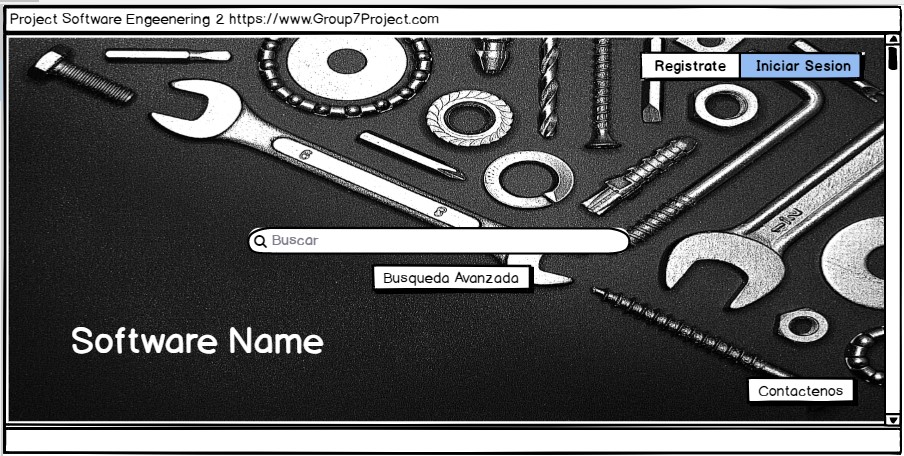
\includegraphics[scale = 0.7]{images/PaginaPrincipal.jpg}
    \caption{Pagina Principal}
    \label{F100}
\end{figure}{}

\begin{figure}[H]
    \centering
    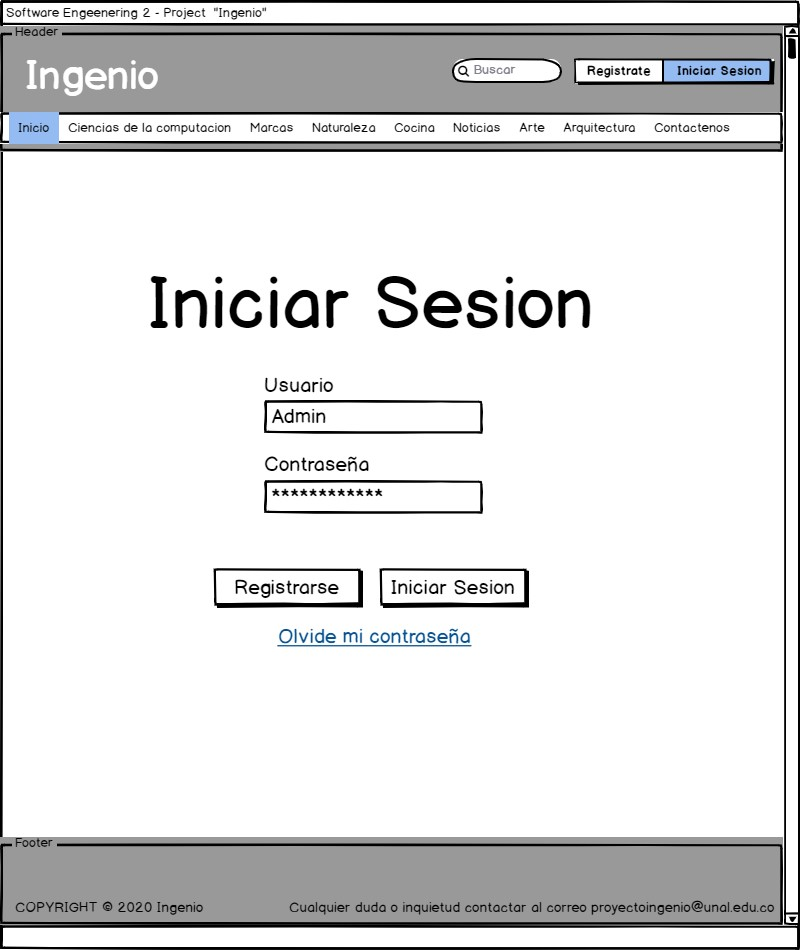
\includegraphics[scale = 0.7]{images/IniciarSesion.jpg}
    \caption{Iniciar Sesión}
    \label{F101}
\end{figure}{}

\begin{figure}[H]
    \centering
    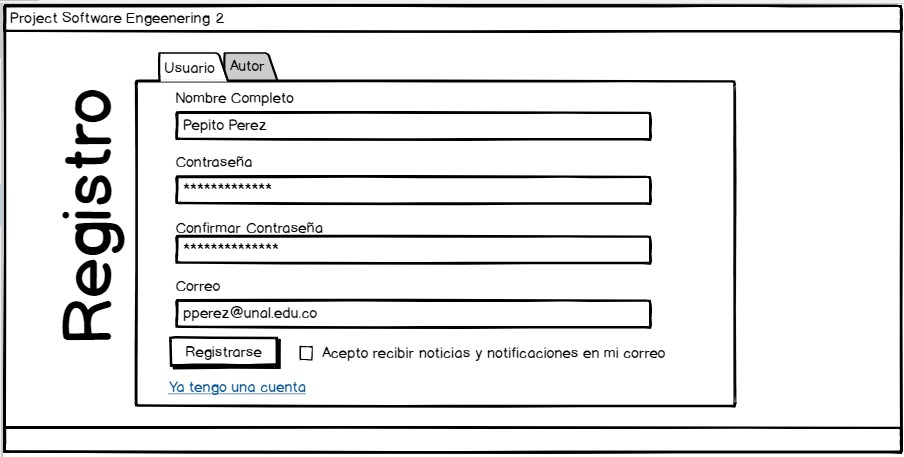
\includegraphics[scale = 0.7]{images/RegistrarseUsuario.jpg}
    \caption{Registrarse Usuario}
    \label{F102}
\end{figure}{}

\begin{figure}[H]
    \centering
    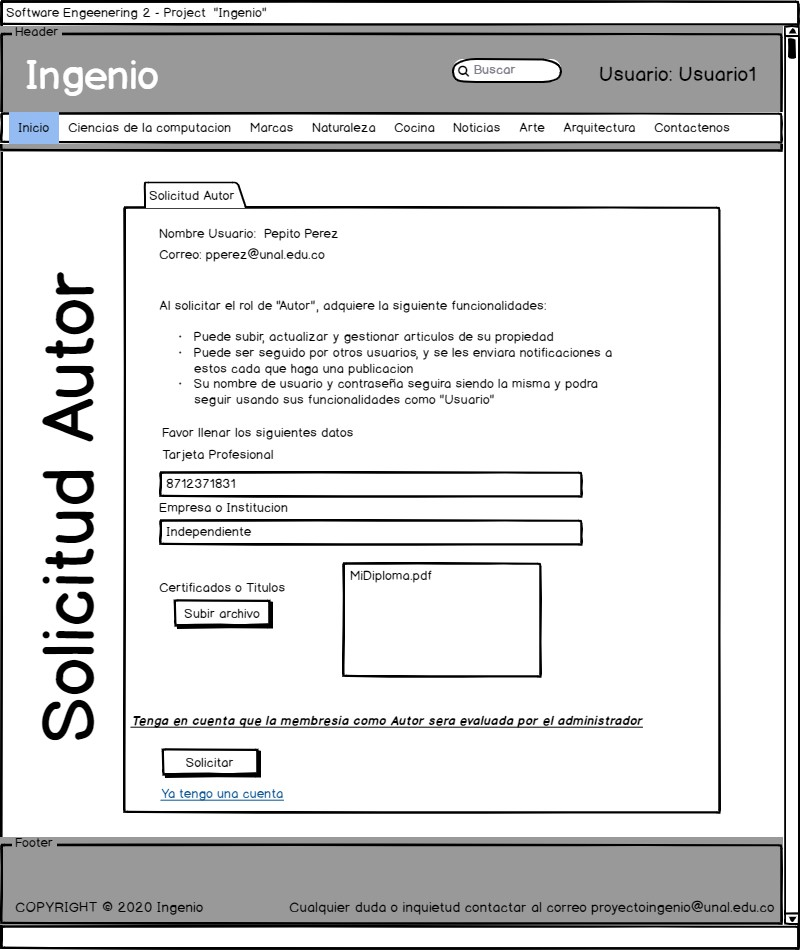
\includegraphics[scale = 0.7]{images/SolicitudAutor.jpg}
    \caption{Solicitud Autor}
    \label{F103}
\end{figure}{}

\begin{figure}[H]
    \centering
    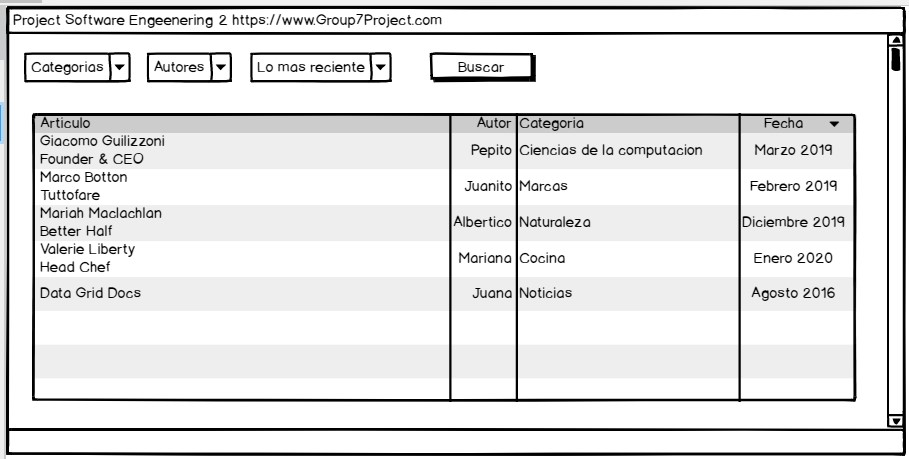
\includegraphics[scale = 0.7]{images/BusquedaAvanzada.jpg}
    \caption{Búsqueda Avanzada}
    \label{F104}
\end{figure}{}

\begin{figure}[H]
    \centering
    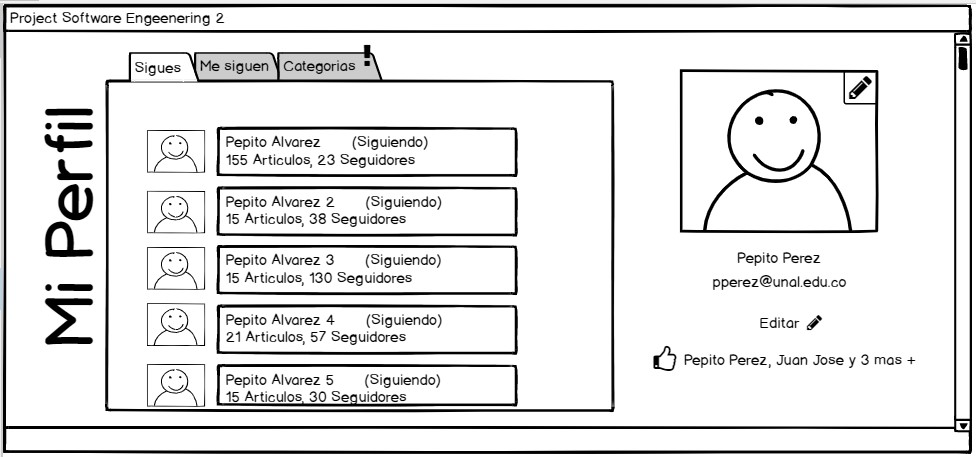
\includegraphics[scale = 0.7]{images/PerfilPropioUsuario.jpg}
    \caption{Perfil Propio Usuario}
    \label{F105}
\end{figure}{}

\begin{figure}[H]
    \centering
    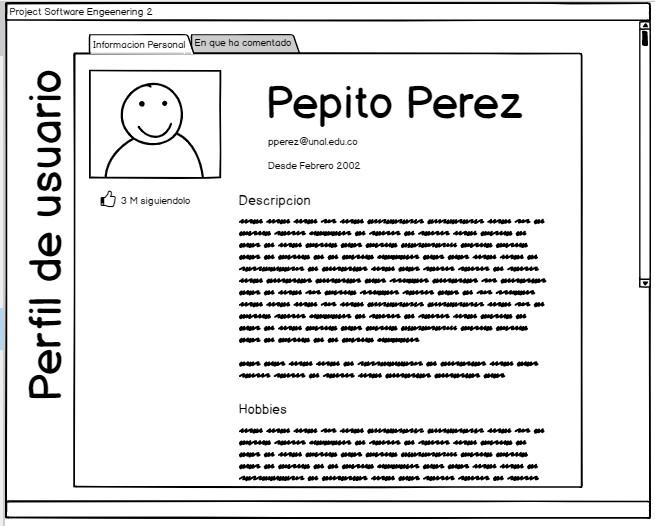
\includegraphics[scale = 0.7]{images/PerfilOtroUsuario.jpg}
    \caption{Perfil Otro Usuario}
    \label{F106}
\end{figure}{}

\begin{figure}[H]
    \centering
    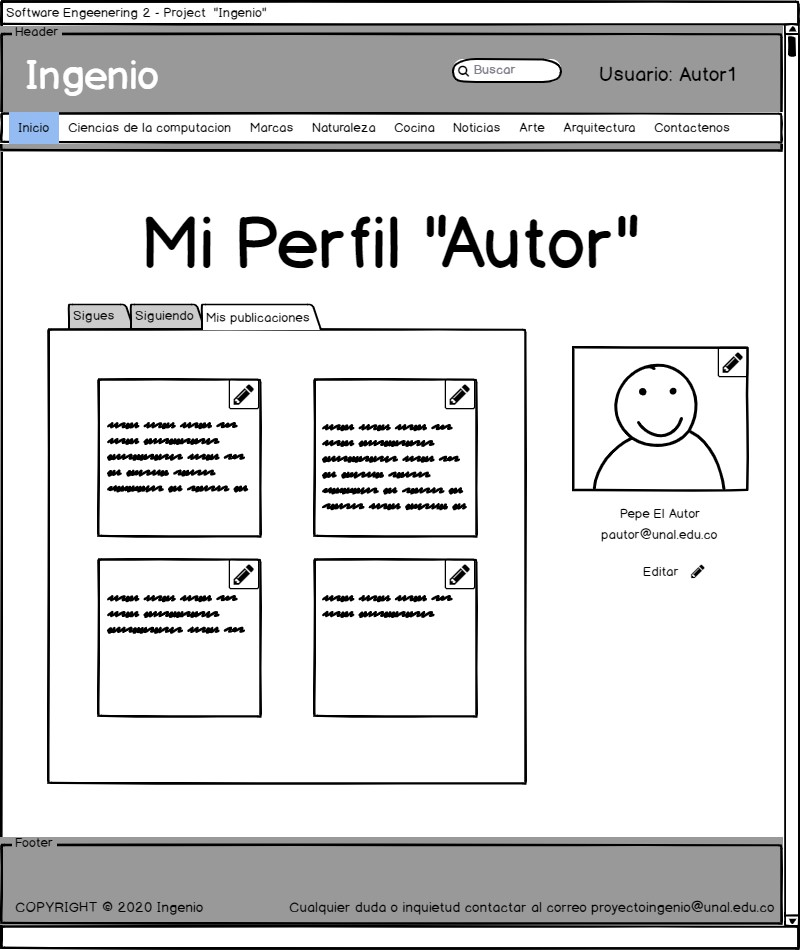
\includegraphics[scale = 0.71]{images/PerfilPropioAutor.jpg}
    \caption{Perfil Propio Autor}
    \label{F107}
\end{figure}{}

\begin{figure}[H]
    \centering
    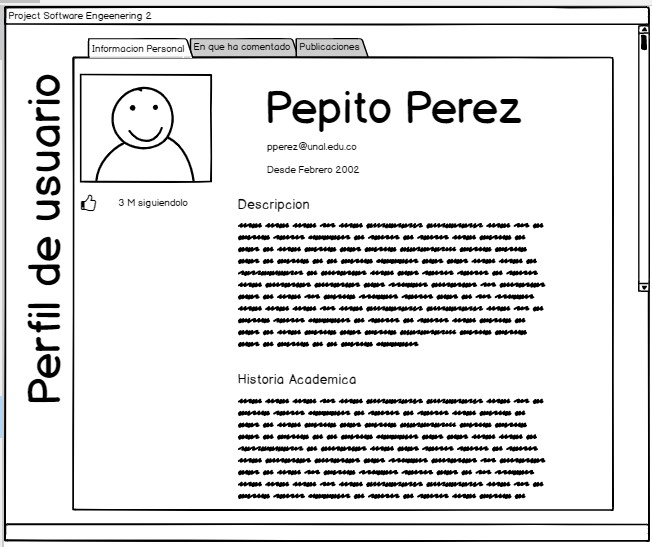
\includegraphics[scale = 0.7]{images/PerfilOtroAutor.jpg}
    \caption{Perfil Otro Autor}
    \label{F108}
\end{figure}{}

\begin{figure}[H]
    \centering
    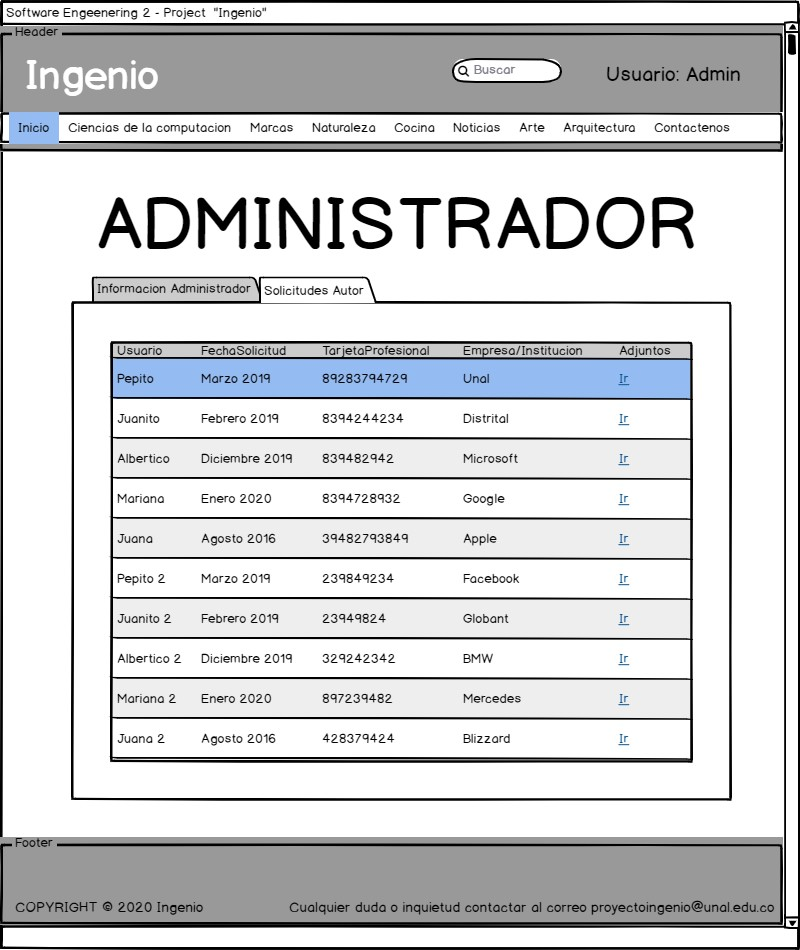
\includegraphics[scale = 0.7]{images/PerfilAdministrador.jpg}
    \caption{Perfil Administrador}
    \label{F109}
\end{figure}{}

\begin{figure}[H]
    \centering
    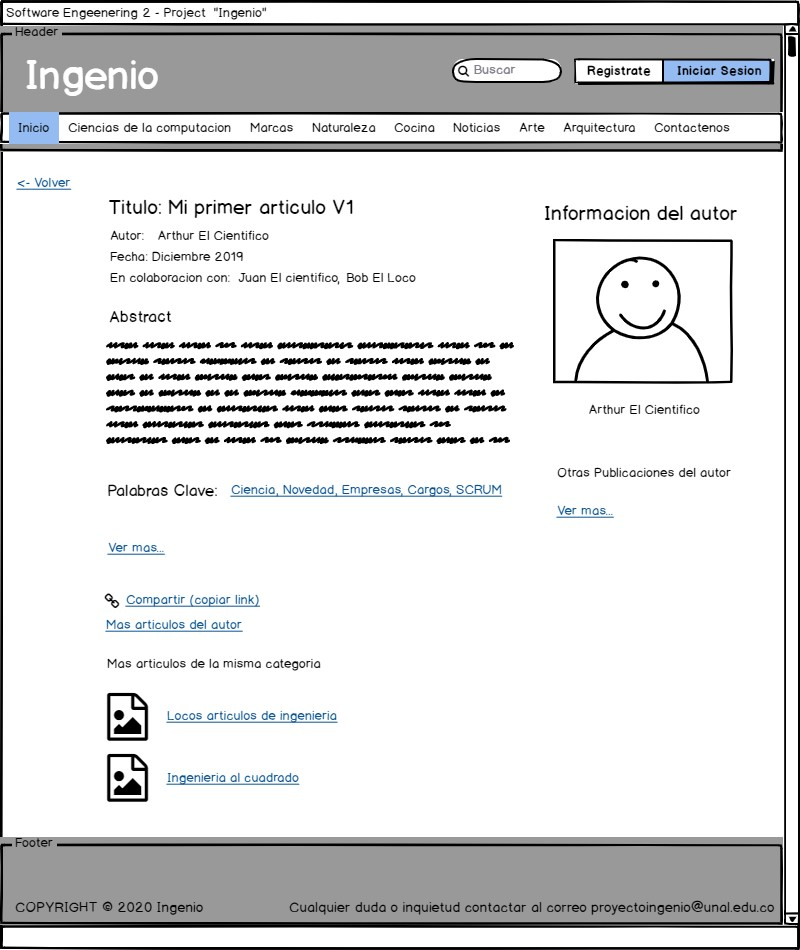
\includegraphics[scale = 0.7]{images/PublicacionVisitante.jpg}
    \caption{Publicación Visitante}
    \label{F110}
\end{figure}{}

\begin{figure}[H]
    \centering
    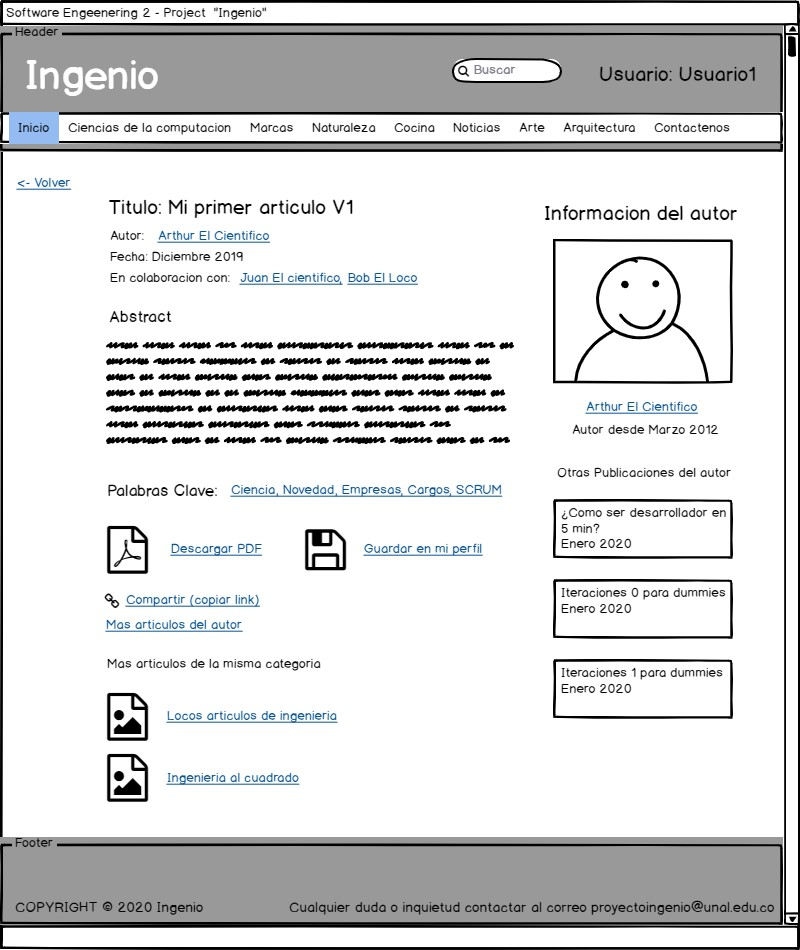
\includegraphics[scale = 0.7]{images/Publicacion.jpg}
    \caption{Publicación}
    \label{F111}
\end{figure}{}

\begin{figure}[H]
    \centering
    
\includegraphics[scale = 0.7]{images/Contactenos.jpg}
    \caption{Contactenos}
    \label{F112}
\end{figure}{}

\begin{landscape}
\section{Modelo Entidad Relación}
    \begin{figure}[H]
        \centering
        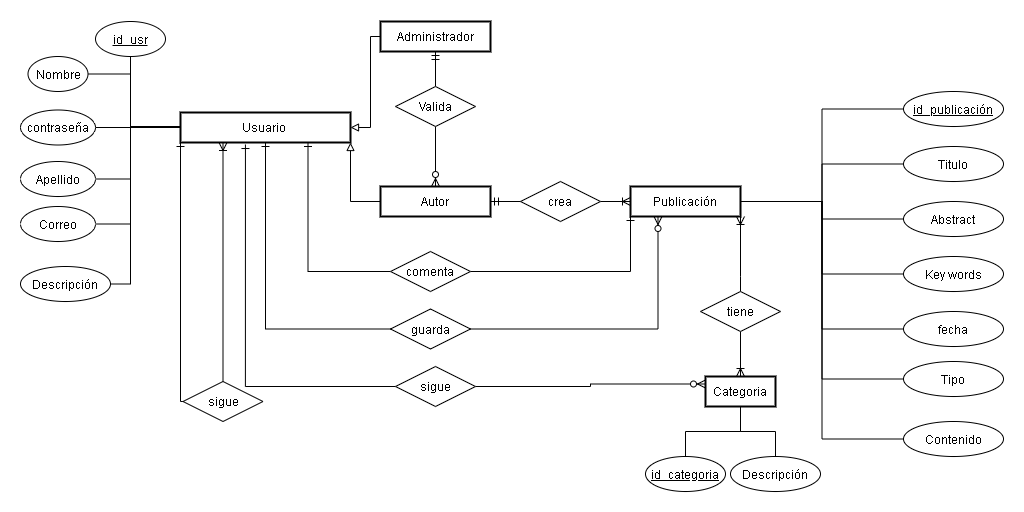
\includegraphics[scale = 0.7]{images/ERD_v02.png}
        \caption{Diagrama modelo ER.}
        \label{F13}
    \end{figure}{}

\section{Modelo de Base de Datos}
    \begin{figure}[H]
        \centering
        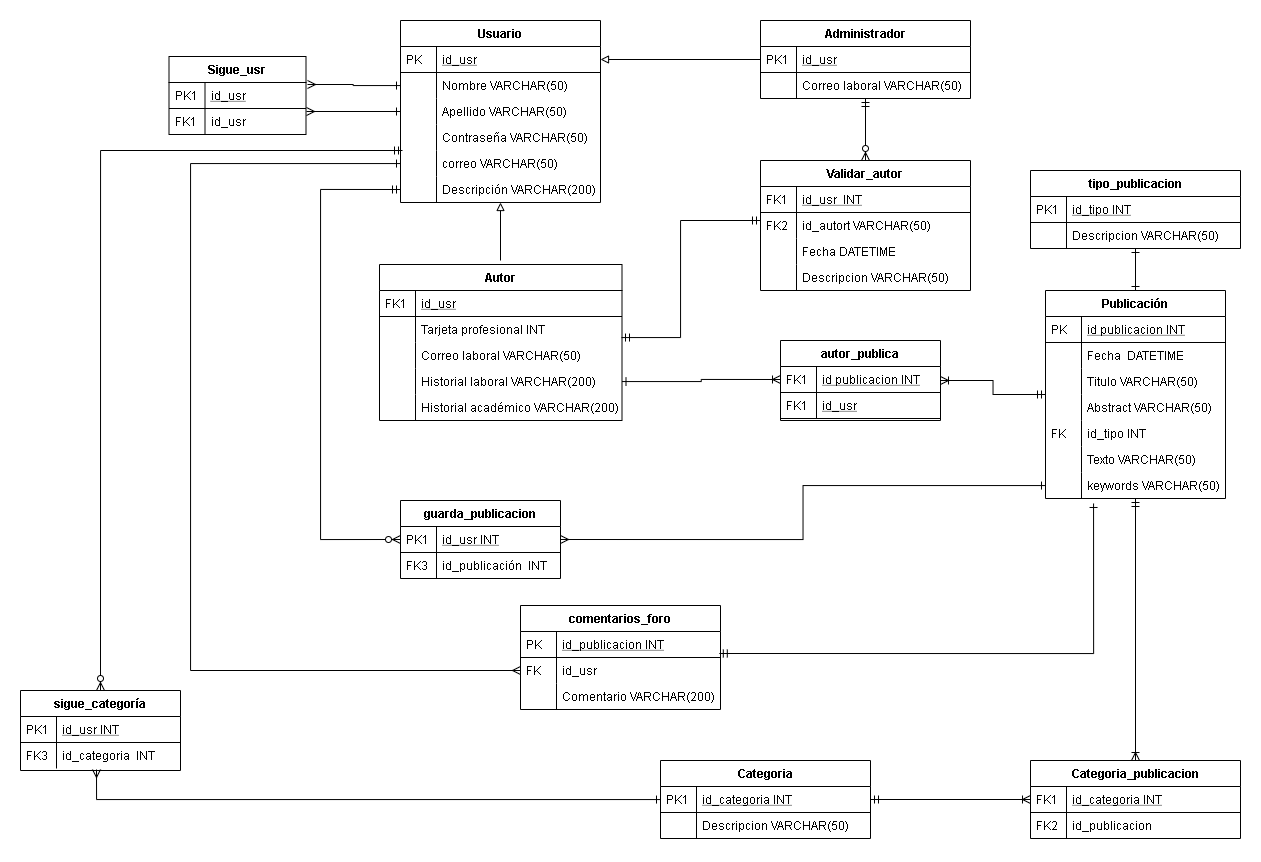
\includegraphics[scale = 0.55]{images/BD_v02.png}
        \caption{Diagrama modelo BD}
        \label{F11}
    \end{figure}{}
\end{landscape}

\section{Estimación de Costos}
El tiempo estimado para realizar el proyecto es del 25 de Marzo del 2020 al 25
de Junio del 2020 (3 meses). \textbf{Por lo tanto todos los gastos se contemplan
para este tiempo estimado}.\\

\textbf{Costos Directos de Personal:}

Los costos directos de personal hacen referencia a las personas contratadas que
colaboran directamente en el proyecto; Scrum Master y 3 desarrolladores.\\

Según la página de búsqueda de empleos “Indeed” \cite{01}, el salario promedio
de un desarrollador de Software en Colombia es de \$ 2’383.039 COP al mes y para
un Scrum Master es de \$3.942.313 .Tanto el Scrum Master, como los
desarrolladores, se encuentran en últimos semestres de universidad, al momento
realizar el proyecto y sus contratos serán al termino de prestación de
servicios. 

% plantilla: copiar y pegar
\begin{table}[H]
    \centering
    \small{
    \begin{tabular}{R{6cm}L{6cm}}
        \textbf{Concepto}   &\textbf{Valor(3 meses)}\\
        \\
        \multicolumn{2}{c}{Scrum master  \dotfill  \$11'826.939} \\
        \multicolumn{2}{c}{Desarrolladores x 3  \dotfill \$21'447.351} \\
        \hline
        \multicolumn{2}{c}{\textbf{Total} \dotfill \$33'274.290} \\
    \end{tabular}
    \label{T04}}
\end{table}{}


\textbf{Costos Indirectos de Personal:}


Los costos indirectos de personal son las personas contratadas que no aportan
directamente al proyecto pero que son necesarias para realizar el trabajo.

Se contratara personal de aseo para hacer la limpieza en la oficina dos veces al
mes, y se le pagara \$ 30.000 COP / día.

\begin{table}[H]
    \centering
    \small{
    \begin{tabular}{R{6cm}L{6cm}}
        \textbf{Concepto}   &\textbf{Valor(3 meses)}\\
        \\
        \multicolumn{2}{c}{Personal de Aseo  \dotfill  \$180.000} \\
        \hline
        \multicolumn{2}{c}{\textbf{Total} \dotfill \$180.000} \\
    \end{tabular}
    \label{T201}}
\end{table}{}

\textbf{Costos Directos de Material:}

Estos costos son los relacionados a la compra o alquiler de equipos necesarios 
para el desarrollo del software, para este proyecto consideramos el alquiler de 
4 computadores \cite{02} por un valor mensual de \$220.000 COP / cada uno,
además se consideran 
el consumo de internet y energía eléctrica en el lugar de desarrollo, estos
corresponden a un valor de \$110.000 COP/mensual de servicio 
de energía eléctrica y \$103.000 COP / mensual por servicio de internet, también
se contempla la compra de mueblería a usar, que consta de 4 escritorios y 4
sillas, por valor de \$2'000.000 COP.

\begin{table}[H]
    \centering
    \small{
    \begin{tabular}{R{6cm}L{6cm}}
        \textbf{Concepto}   &\textbf{Valor(3 meses)}\\
        \\
        \multicolumn{2}{c}{Alquiler de equipos x 4  \dotfill  \$2'640.000} \\
        \multicolumn{2}{c}{Servicio de energía eléctrica\dotfill  \$330.000} \\
        \multicolumn{2}{c}{Servicio de internet \dotfill \$309.000} \\
        \multicolumn{2}{c}{Compra Mueblería \dotfill \$2'000.000} \\
        \hline
        \multicolumn{2}{c}{\textbf{Total} \dotfill \$5'279.000} \\
    \end{tabular}
    \label{T03}}
\end{table}{}

\textbf{Costos Indirectos de Material:}

Estos costos son los no relacionados directamente con el proyecto, pero
necesarios en el ambiente de trabajo. Tales como, recibo de agua por un valor
mensual de \$120.000 COP, además implementos de aseo que corresponden a un valor
de \$150.000 COP/mensual y gastos varios o de papelería por \$50.000 COP /
mensual.

\begin{table}[H]
    \centering
    \small{
    \begin{tabular}{R{6cm}L{6cm}}
        \textbf{Concepto}   &\textbf{Valor(3 meses)}\\
        \\
        \multicolumn{2}{c}{Servicio de agua \dotfill  \$360.000} \\
        \multicolumn{2}{c}{Implementos de aseo 
        \dotfill  \$450.000} \\
        \multicolumn{2}{c}{Papelería y varios
        \dotfill \$150.000} \\
        \hline
        \multicolumn{2}{c}{\textbf{Total} \dotfill \$960.000} \\
    \end{tabular}
    \label{T203}}
\end{table}{}

\textbf{Total de Costos:}

En esta sección se encuentra el resumen de todos los costos del proyecto, y el
valor final a cobrar.

\begin{table}[H]
    \centering
    \small{
    \begin{tabular}{R{6cm}L{6cm}}
        \textbf{Concepto}   &\textbf{Valor(3 meses)}\\
        \\
        \multicolumn{2}{c}{Costos directos personal  \dotfill  \$33'274.290} \\
        \multicolumn{2}{c}{Costos indirectos personal  \dotfill  \$180.000} \\
        \multicolumn{2}{c}{Costos directos de material \dotfill \$5'279.000} \\
        \multicolumn{2}{c}{Costos indirectos de material \dotfill \$960.000} \\
        \hline
        \multicolumn{2}{c}{\textbf{Total (antes de instalación)} 
        \dotfill \$39'693.290} \\
        \multicolumn{2}{c}{Instalación \dotfill \$500.000} \\
        \hline
        \multicolumn{2}{c}{\textbf{Total (antes de ganancia esperada)} 
        \dotfill \$40'193.290} \\
        \multicolumn{2}{c}{Ganancia esperada (20\%) \dotfill \$8'038.658} \\
        \hline
        \multicolumn{2}{c}{\textbf{Total (Precio mínimo)} 
        \dotfill \$48'231.948} \\
        \multicolumn{2}{c}{Ajuste Final \dotfill - \$231.948} \\
        \hline
        \multicolumn{2}{c}{\textbf{Total Esfuerzo Nominal} 
        \dotfill \$48'000.000} \\
        \multicolumn{2}{c}{Esfuerzo de sobrecarga (50\%) 
        \dotfill - \$24'000.000} \\
        \hline
        \multicolumn{2}{c}{\textbf{Costo Total} \dotfill \$72'000.000} \\
    \end{tabular}
    \label{T205}}
\end{table}{}

Se estima un valor total \$72'000.000 COP por el costo total del proyecto.


\section{Análisis de riesgos}


\begin{table}[H]
    \centering
    \small{
    \begin{tabular}{|M{1cm}|M{3cm}|M{10cm}|}
        \hline
        \textbf{Valor}  &\textbf{Tipo}   &\textbf{Definición}\\
        \hline 
            1   & Técnico
            & Daños o problemas con los dispositivos que intervienen en el
            desarrollo de la aplicación.\\
        \hline
            2  & Organizacional
            & Errores en la ejecución de diferentes planes de trabajo por parte
            de los individuos que intervienen en el desarrollo de la aplicación.
            \\
        \hline
            3   & Cronograma
            & Contratiempos que afectan el desarrollo de actividades en el
            tiempo estimado.      \\
        \hline
            4   & Externo
            & Problemas que son ajenos a la organización.    \\
        \hline
            5   & Gerencial
            & Malas prácticas que provocaron la creación de modelos de trabajo
            inadecuados para el desarrollo de la aplicación.   \\
        \hline
    \end{tabular}
    \caption{Tipos de riesgo}
    \label{Riesgo3}}
\end{table}{}


\begin{table}[H]
    \centering
    \small{
    \begin{tabular}{|M{1cm}|M{2cm}|M{11cm}|}
        \hline
        \textbf{Valor}   &\textbf{Significado}   &\textbf{Criterio}\\
        \hline 
            1   & Muy bajo
            & No afecta el desarrollo, calidad o esencia de la aplicación, ni
            altera el tiempo de ejecución estimado para las siguientes etapas de
            trabajo.\\
        \hline
            2   & Bajo
            & Afecta en pequeña medida la esencia, calidad de la aplicación o el
            cronograma predefinido para cada fase de desarrollo. \\
        \hline
            3   & Moderado
            & Afecta en una medida considerable el cronograma predefinido de
            desarrollo, la calidad de la aplicación o su esencia.  \\
        \hline
            4   & Alto
            & Afecta en gran medida el desarrollo de la aplicación y es
            necesario y redefinir modelos de trabajo para continuar con el
            proyecto.      \\
        \hline
            5   & Muy alto
            & El impacto sobre el cronograma o la aplicación es muy alta y es
            imposible crear un modelo de trabajo que permita retomar el trabajo
            con los recursos disponibles.\\
        \hline
    \end{tabular}
    \caption{Niveles de Impacto}
    \label{Nimpacto}}
\end{table}{}

\small{
\centering
\begin{longtable}{|M{4cm}|M{1cm}|M{1.5cm}|M{2.5cm}|M{6cm}|}
    \endfirsthead
    \multicolumn{5}{c}%
    {{\tablename\ \thetable{} -- Continúa de la página anterior}} \\
    
    \hline
    \textbf{Riesgo} & \textbf{Tipo} &\textbf{Impacto}
    & \textbf{Probabi-lidad} & \textbf{Plan de acción}\\
    \hline
    \endhead
    
    \hline
    \multicolumn{5}{c}{{\tablename\ \thetable{} -- Continúa en la siguiente
    página.}} \\ 
    \endfoot
    \endlastfoot
    
    \hline
    \textbf{Riesgo} & \textbf{Tipo} &\textbf{Impacto}
    & \textbf{Probabilidad} & \textbf{Plan de acción}\\
    \hline
    Un integrante del equipo de desarrollo renuncia.
    & 4 & 3  & 10\%  
    & Distribuir el trabajo del desarrollador entre los
    demás miembros del equipo y evaluar si es necesario replantear la
    entrega prevista.\\
    \hline
    Perdida de herramientas de comunicación de desarrollo tales como internet.
    & 4 &  4 &   4\%
    &  Entrega de paquetes de avance de trabajo periódicamente y coordinado por
    cualquier otro medio de comunicación. \\
    \hline
    El hardware del equipo no cumple con los requerimientos mínimos para
    culminar el desarrollo del proyecto.
    & 3 & 3  & 5\%  
    & Se buscara un hardware que solucione esta necesidad para la culminación
    del proyecto . \\
    \hline
    La planificación del desarrollo de historias de usuario no están bien
    coordinadas.
    & 2 &  4 & 15\%  
    &  Programar las tareas de desarrollo\\
    \hline
    Una tarea requiere mas tiempo de lo esperado.
    & 3 &  3 & 17\%   
    &  Destinar mas horas de trabajo y equipo de  desarrollo para terminar la
    tarea. \\
    \hline
    El proyecto es cancelado por motivos extracurriculares
    & 4 & 5  & 6\%  
    &  Decidir si culminar o no el proyecto \\
    \hline
    La metodología de desarrollo no ofrece el desempeño esperado.
    & 5 & 2  & 15\%
    &  Dado el caso se repensara la implementación de cierta metodología para
    próximos proyectos.  \\
    \hline
    El software presenta errores tiempo después de haber sido completado en
    iteraciones anteriores.
    & 1 & 3  & 30\%  
    & Se hará una revisión de los cambios hasta donde no ocurrían los errores
    solucionados o se decidirá corregirlos juntamente con los cambios realizados
    \\
    \hline
    El scrum master no cumple con lo requerido para mantener al equipo de
    desarrollo activo y entorno saludable.
    & 2 & 1  &  15\%
    &  Cambio del scrum master por algún otro integrante del equipo  \\
    \hline
    Los tiempos de entrega se ven reducidos
    & 3 &  4 & 5\%  
    &  Reprogramación de tareas por cada historia de usuario restante \\
    \hline
    Cambio de objetivo del proyecto por parte del cliente
    & 4 & 5  & 15\%  
    & Replanteamiento de historias de usuario y buscar homologación del trabajo
    realizado  \\
    \hline
    Priorización inadecuada en la gestión de proyectos.
    & 5 & 2  & 20\%
    & Buscar nuevas formas de organizar las tareas en siguientes iteraciones. \\
    \hline
    \caption{Riesgos de desarrollo.} 
    \label{Riesgos}
\end{longtable}}


\section {Comparación Frameworks }

Para la elección de Frameworks que serán usados en el desarrollo del proyecto se realizo una comparación, entre diferentes entornos de trabajo tanto para Back End y Front End, considerando: su popularidad, la disponibilidad de recursos de aprendizaje y sus funciones principales, mostrando sus ventajas y desventajas.\\

\textbf{FrontEnd}:\\

Para la elección de frameworks en FrontEnd se tuvo en cuenta, \textbf{React}, \textbf{Angular} y \textbf{Vue}.\\

Inicialmente fueron considerados estos tres entornos dada su popularidad, ya que son de las herramientas más usadas en la actualidad, por lo tanto cuentan con una gran comunidad de desarrolladores, lo cual nos permite contar con mayor información y dada la antigüedad de algunos, se podría tener mas oportunidades en el ámbito laboral (React y Angular), en la siguiente tabla se muestra la información correspondiente a la popularidad de estos entornos. 

\begin{table}[H]
    \centering
    \small{
    \begin{tabular}{|M{5cm}|M{2.5cm}|M{2.5cm}|M{2.5cm}|}
        \hline
         &\textbf{Angular}   &\textbf{React} &\textbf{Vue Js}\\
        \hline 
            Stars on GitHub   & 26,924
        & 73,530 & 63,438
            \\
        \hline
            Contributors on GitHub & 495
        & 1044 & 122
            \\
        \hline
            Tagged questions on StackOverflow  & 66,152
        & 54,158 & 8598
            \\
        \hline
    \end{tabular}
    \caption{Popularidad, Tomado de \cite{03}}
    \label{Riesgo}}
\end{table}{}

Respecto a las funciones principales, todas tiene características que permiten destacar cada una de las herramientas; como por ejemplo Angular,que permite desde su entorno trabajar procesamiento y validación de formularios y comunicación HTTP, por el contrario estas son tareas que en React y Vue dependen del desarrollador, a continuación se muestra una tabla con las ventajas y desventajas de cada Framework.

\begin{table}[H]
    \centering
    \small{
    \begin{tabular}{|M{2.5cm}|M{6.5cm}|M{6.5cm}|}
        \hline
        \textbf{Framework}  &\textbf{Ventajas}   &\textbf{Desventajas}\\
        \hline 
            React   &
            \begin{itemize}
                \item Alto desempeño.
                \item Adecuado para aplicaciones con mucho tráfico.
                \item DOM virtual(enlace de datos unidireccional).
            \end{itemize}   &
            \begin{itemize}
                \item Necesita otras librerías para construir aplicaciones complejas.
            \end{itemize}
            \\
        \hline
            Angular & 
            \begin{itemize}
                \item Enlace de datos bidireccional
                \item Aplicación simple de una pagina.
                \item Permite procesamiento y validación de formularios.

            \end{itemize}   &
            \begin{itemize}
                \item Se debe aprender Typescript.
                \item Complejo y difícil de aprender.
            \end{itemize}
            \\
        \hline
            Vue.js  & 
            \begin{itemize}
                \item Alto desempeño. 
                \item Flexibilidad. 
                \item DOM visual y basado en componentes
            \end{itemize}   &
            \begin{itemize}
                \item El más joven del los entornos 
                \item Poco mercado.
                \item Ser demasiado flexible puede generar problemas
            \end{itemize}
            \\
        \hline
            
    \end{tabular}
    \caption{Frameworks FrontEnd}
    }
\end{table}{}

Considerando la información anterior, seleccionamos Vue JS como framework FrontEnd, ya que es uno de los más fáciles de aprender y se adapta fácilmente en la creación de interfaces de usuario además proporciona un período de cambio rápido de otros frameworks a Vue.js debido a la similitud con Angular y React en términos de diseño y arquitectura.\\

\textbf{BackEnd}:\\

Para realizar la comparacion de frameworks en Back End, decidimos analizar algunos de los mas usados y conocidos actualmente, \textbf{Sprint (Java)}, \textbf{Django (Python)} y \textbf{Node JS (Javascript)}.\\


\begin{table}[H]
    \centering
    \small{
    \begin{tabular}{|M{2.5cm}|M{6.5cm}|M{6.5cm}|}
        \hline
        \textbf{Framework}  &\textbf{Ventajas}   &\textbf{Desventajas}\\
        \hline 
            Spring   & 
            \begin{itemize}
                \item Buena separación entre componentes de front-end y la lógica de Java.
                \item Desarrollo orientado a componentes estilo SWING
                \item Facil de debuggear
                \item Su uso son Java y HTML simples, los conceptos de Java se utilizan a gran nivel
            \end{itemize}   & 
            \begin{itemize}
                \item Se actualiza muy constantemente, y esto puede causar problema con versiones nuevas
                \item Entre mas componentes tiene una pagina, mas complejo y desorganizado se vuelve el codigo
                \item Limitado a pagina simples
                \item Documentacion actalizada escaza
            \end{itemize}
            \\
        \hline
            Django & 
            \begin{itemize}
                \item Django fue creado para trabajar bajo un patrón MVC (Modelo Vista Controlador) quien se encarga del manejo de controladores, esto lo caracteriza en un framework reusable y permite el desarrollo ágil.
                \item Según la comunidad que desarrolla bajo Python, los API’s REST que genera Django son mucho mejores, debido a que se pueden convertir en páginas HTML como puntos finales (Endpoints).
                \item Tiene un panel de administración para gestionar bases de datos.
            \end{itemize}   &
            \begin{itemize}
                \item A pesar de su excelente documentación, es muy extensa y tiende a ser confusa.
                \item A la hora de realizar un API REST conlleva cierta condición de dificultad a comparación de Flask.
                \item La implementación de sockets es algo compleja de usar.
            \end{itemize}
            \\
        \hline
            Node.js  &
            \begin{itemize}
                \item Si tu aplicación no tiene ningún cálculo intensivo del CPU, puedes construir en Javascript de arriba a abajo, inclusive a nivel de base de datos si utilizas el objeto de almacenamiento JSON como MongoDB DB. Esto facilita el desarrollo (incluyendo la contratación) significativamente.
                \item Los Crawlers reciben una respuesta totalmente HTML, que es mucho más SEO-friendly, digamos, una sola página o en una aplicación de Websockets app se ejecuta sobre Node.js.
            \end{itemize}   &
            \begin{itemize}
                \item • Un CPU de cálculo intensivo bloqueará la receptividad del Node.js, por lo que una plataforma de roscado es un mejor enfoque. Alternativamente, podrías intentar escalar el cómputo.
                \item • Utilizando Node.js con una base de datos relacional es aún bastante doloroso (leer más abajo para ver más detalles). Hazte un favor y escoge cualquier otro entorno como Rails, Django, o ASP.NET MVC si estás intentando realizar operaciones relacionales.
            \end{itemize}
            \\
        \hline
            
    \end{tabular}
    \caption{Frameworks BackEnd}
    }
\end{table}{}

Segun la comparacion de estos tres llegamos a la eleccion de \textbf{NODE JS}.\\

Ya que la eleccion para Front End fue  Vue JS, recurrimos a la tarea de analizar los Stacks mas usados y pedidos dentro de la industria de software que se relacionaran de mejor manera a estos frameworks.\\

Al buscar esto, encontramos que los mas usados son:\\ 

\textbf{Stack MEAN}:

MongoDB, Express, AngularJS y Node.js\\

\textbf{Stack MERN}:

MongoDB, Express, React y Node.js\\

Lo que nos llevo a encontrar:

\textbf{Stack MEVN}:

MongoDB, Express, Vue y Node.js\\


El cual funciona de la siguiente forma:
\begin{itemize}
\item MongoDB: servicio de gestión de bases de datos multiplataforma orientado a documentos (conjunto de registros o de datos) y de esquema totalmente libre (no debe estar predefinido). Así, cada documento puede tener atributos distintos al resto.
\item Vue JS: marco de desarrollo de front-end. Es un framework de JavaScript de código abierto y libre, que permite el desarrollo de aplicaciones web en el lado del cliente.
\item Node.js: entorno de desarrollo en la capa del servidor. Su objetivo es que un programador sea capaz de desarrollar una aplicación con altos niveles de escalabilidad en una única máquina, aunque las peticiones de usuarios y clientes no dejen de aumentar con el tiempo.  La lógica apunta a la fórmula ‘más clientes, más coste’, pero Node.js rompe esa ecuación.
\item Express: framework para el desarrollo de back-end. Es un marco de desarrollo rápido, flexible y con una gran comunidad detrás, lo cual siempre es importante por el volumen de documentación existente para el desarrollo de proyectos.
\end{itemize}

Y este el ultimo \textbf{sera el Stack que se usara para realizar el desarrollo} de "Ingenio". Otro factor importante para la eleccion de este Stack, es la programacion usando un solo lenguaje (Javascript) tanto para Front End y Back End.

%%%Escribir justificacion
\section{Repositorio }

\begin{itemize}
    \item BackEnd
    \item FrontEnd
\end{itemize}

\section{Sprint 1}

\section*{Tablero Kanban}
\section*{Slack} 
\section*{Hash Spritn 1}
\begin{itemize}
    \item BackEnd
    \item FrontEnd
\end{itemize}


\begin{thebibliography}{50}
\bibitem{01} Indeed Salarios. Disponible en: 
\url{https://co.indeed.com/salaries/desarrollador-de-software-Salaries}
\bibitem{02} Renta sistemas. Disponible en:\url{https://www.rentasistemas.com/}

\bibitem{03}Adictec, Cómo Elegir el Mejor Framework de Front-End.
Disponible en:\url{https://adictec.com/como-elegir-el-mejor-framework-de-front-end/}
\documentclass[a4paper,12 pt]{article}

%% Language and font encodings
\usepackage[spanish,es-tabla]{babel}
\usepackage[utf8]{inputenc}
\usepackage[T1]{fontenc}
\usepackage{cite}
\usepackage{amsmath, amsthm, amssymb, amsfonts} 
\usepackage[mathscr]{eucal}
\usepackage{ulem} % subrayar, tachar
\usepackage{hyperref} % para el url
\usepackage{multirow, array} % para las tablas
\usepackage{float} % para tablas [H]
\usepackage{graphicx} % graficos
\usepackage{titlesec} %subsubsubsection
\usepackage[usenames]{color} %palabras con color
\usepackage{lscape} % texto horizontal
\usepackage{pdflscape} % hoja horizontal
\usepackage{booktabs} %tabla con puntos
\usepackage{longtable} 

\newcolumntype{P}[1]{>{\centering\arraybackslash}p{#1}}
\newcolumntype{M}[1]{>{\centering\arraybackslash}m{#1}}
\newcolumntype{L}[1]{>{\raggedleft\arraybackslash}p{#1}}
\newcolumntype{R}[1]{>{\raggedright\arraybackslash}p{#1}}
  
%counter
\newcounter{mycounter} % create a new counter, called 'mycounter'
% default def'n of '\themycounter' is '\arabic{mycounter}'

%% command to increment 'mycounter' by 1 and to display its value:
\newcommand\showmycounter{\stepcounter{mycounter}\themycounter}

\usepackage{lipsum}
\newcommand\showlips{\stepcounter{mycounter}\lipsum[\value{mycounter}]}

%ppppppppppppppppppppppppppppppppppppppppppppppppppppppppppppppppppppppppppppppp

%% Sets page size and margins
\usepackage[a4paper,top=2cm,bottom=2cm,left=2cm,right=2cm,marginparwidth= 1.5cm]{geometry}
  
\title{\LARGE \textbf{\\[0.5cm] IngenioUN\\[2.5cm]}}

% Chicos, porfavor incluyan sus nombres en orden alfabetico
\author{\textbf{Grupo 7}\\[0.5cm]
        Valeria Huepa Ducuara\\
        Juan José Peña Becerra\\
        Carlos Daniel Rincón Mora\\
        Guiselle Tatiana Zambrano Penagos\\[2.5cm]
        Sebastian David Moreno Bernal\\[2.5cm]}
\date{}

\begin{document}

\newpage

\begin{figure}
    \centering
    
\includegraphics[width=0.57\textwidth]{images/escudoUN.png}
\end{figure}
\maketitle 
\thispagestyle{empty}

\begin{center}
    \small Universidad Nacional de Colombia\\
    Facultad de Ingeniería\\
    Departamento de Ingeniería de Sistemas e Industrial\\
    Ingeniería de Sistemas\\
    Ingeniería de Software II\\
    Bogotá, Colombia\\
    2020
\end{center}
\newpage
\tableofcontents % indice de contenidos}
\thispagestyle{empty}

\newpage
\setcounter{page}{1}
\pagestyle{plain}

\section{Descripción General}


\subsection{Descripción del Problema}

Dada la existencia de una necesidad de tener una plataforma online,
adicionalmente no existen muchos canales de información para personas
interesadas en el campo de la Ingeniería que quieran mantenerse informadas
diariamente por medio de informes, artículos y noticias de parte de una fuente
confiable y en constante actualización, esto es porque los canales existentes no
se mantienen en continuo mantenimiento o no son de agrado para el público en
mención. Así mismo, hoy en día circulan noticias falsas por redes sociales, y en
otros medios de comunicación quitando la certeza y veracidad de la información.
Se desea una plataforma más personal, en donde las personas del campo de la
Ingeniería pueden conocerse e interactuar entre ellas, para obtener conocimiento
en diversas áreas en común de interés para cada uno, además de comentar a los
demás usuarios su opinión de cierto tema.\\

\subsection{Descripción del Producto}

El software a realizar pretende tener un vínculo con el público interesado en
temas actuales de Ingeniería (Stakeholders), y desea brindarle información de
primera mano, así como artículos (científicos, de opinión y periodísticos ) de
gran interés para el mundo actual, con autores de renombre en la industria de
Ingeniería. Así mismo, podrán registrarse para recibir notificaciones cada que
algún artículo de su posible interés sea publicado. Recibirán notificaciones de
sus autores preferidos, para mantenerse actualizados con el trabajo de
reconocidos ingenieros.\\

Se desea realizar una plataforma más personal, que las que existen actualmente,
en la cual los usuarios puedan conocer a otras personas con intereses similares
en el campo de la Ingeniería, además de conocer, seguir y comentar el trabajo de
otros ingenieros.El registro como usuario es de carácter público, mientras que
para que para ser autor y poder realizar una publicación, esté debe ser aprobado
por el administrador, demostrando conocimiento en un área de interés, presentado
comprobantes de estudios y experiencia académica o laboral.\\

La plataforma cuenta con diferentes foros, en los cuales los usuarios podrán dar
su opinión de forma libre, siempre y cuando sean respetuosos con los demás
usuarios y autores, en caso contrario su cuenta podría ser vetada o eliminada de
la plataforma.

\subsection{Descripción de los Roles de Usuario}

\begin{itemize}
    \item \textbf{Administrador:} Individuo que posee el rol de usuario y
    administrador, este tiene permisos especiales que le permiten, crear nuevas
    categorías otorgar o despojar el rol de autor para los usuarios, este tendrá
    que verificar que el usuario que desee publicar contenido en la plataforma
    posea comprobantes que respalden su experiencia académica y laboral sobre
    uno o varios temas relacionados con la ingeniería, también será el
    responsable de atender las diferentes denuncias realizadas por los usuarios
    y determinar si es pertinente o no vetar o eliminar al usuario denunciado.
    
    \item \textbf{Autor:} Individuo que posee el rol de usuario y autor, este
    puede publicar contenido relacionado con la ingeniería en la plataforma e
    interactuar con los demás usuarios, para publicar información este puede
    hacerlo en formato PDF, JPG o PNG, podrá agregar archivos de opinión,
    investigación y noticias clasificándolos en una o mas categorías
    (computación, electrónica, mecánica, robótica, investigación, noticias y
    opinión) y presentar esta información por medio de infografías, o texto
    plano.
    
    \item \textbf{Usuario:} Es el rol que tendrán todos los individuos que se
    registren en la plataforma, este podrá suscribirse a una o más categorías lo
    que le permitirá tener una sección de cada una en la pantalla de inicio, con
    los diferentes archivos pertenecientes a esta. Este también podrá seguir a
    autores y otros usuarios y recibir notificaciones cada vez que estos
    publiquen archivos de información o realicen comentarios en los foros. Este
    usuario podrá acceder a la información de la plataforma por medio de un
    buscador general (filtrando por palabras clave) o especializada (fecha de
    publicación, autor, categoría y tipo).
    
    \item \textbf{Visitante:} Este podrá ver la pagina principal de noticias y
    acceder al buscador general (filtrando por palabras clave), podrá ver las
    diferentes categorías y acceder a los artículos e infografías, más no podrá
    suscribirse a ninguna categoría, seguir autores o usuarios ni comentar en
    ningún foro. Si este desea acceder a más funcionalidades, tendrá que
    registrarse a la plataforma.
\end{itemize}{}

\section{Descripción del Equipo y Metodología de Desarrollo}

La metodología a seguir en este proyecto es Scrum, siguiendo todas las etapas y
características de la metodología mencionada. El manejo del código de software
se manejará por medio de un sistema de control de versiones central, usando las
herramientas Git y GitHub por parte de cada uno de los desarrolladores. \\

Para el correcto avance del proyecto se realizarán entregas parciales con
análisis de cada aspecto de este. Las fechas de los avances del proyecto serán
de la siguiente manera:

\begin{itemize}
    \item \textbf{Iteración 0:} Marzo 24 del 2020
    \item \textbf{Iteración 1:} Abril 14 del 2020
    \item \textbf{Iteración 2:} Mayo 5 del 2020
    \item \textbf{Iteración 3:} Mayo 26 del 2020
    \item \textbf{Iteración 4:} Junio 16 del 2020
    \item \textbf{Iteración Final:} Junio 23 del 2020
\end{itemize}{}

\subsection{Roles del equipo}

La forma en la que se trabajará durante el desarrollo del software será en
equipos de 2 personas, donde uno de ellos trabajará en el front-end y otro en el
back-end, los equipos serán redefinidos en cada iteración y estos mantendrán
comunicación diaria, mientras que los reportes de avances por equipo serán
realizados 2 veces por semana, donde todos los desarrolladores estarán
presentes.

\begin{table}[H]
    \centering
    \small{
    \begin{tabular}{|c|c|}
        \hline
        \textbf{Rol}   &   \textbf{Nombre}  \\ 
        \hline
        Product Owner   &   Sebastian David Moreno Bernal\\
        \hline
        Scrum Master   &   Guiselle Tatiana Zambrano Penagos\\
        \hline
        \multirow{2}{2cm}{Front End}    &   Valeria Huepa Ducuara\\
            &   Carlos Daniel Rincón Mora\\
        \hline
        \multirow{2}{2cm}{Back End}    &   Juan José Peña Becerra\\
            &   Guiselle Tatiana Zambrano Penagos\\
        \hline
         
    \end{tabular}
    \caption{Roles del equipo}}
    \label{T00}
\end{table}{}

\subsection{Recursos del equipo}

\begin{table}[H]
    \centering
    \small{
    \begin{tabular}{|M{2cm}|M{1.5cm}|M{3cm}|M{3cm}|M{1.5cm}|M{2cm}|}
        \hline
        \textbf{Nombre}    &\textbf{Marca}     &\textbf{Sistema Operativo} 
        &\textbf{Procesador}   &\textbf{RAM}   &\textbf{Capacidad}\\
        \hline
        Valeria Huepa                       &Asus   &Windows 10 Home x64 
        & Intel(R) Core(TM) i5-4210U CPU    &12GB   &HDD 240GB \\
        \hline
        Juan Peña                           &Asus   &Windows 10 Home x64
        &Intel(R) Core(TM) i5-6198DU CPU @ 2.30 GHz &8GB    &HDD 240GB\\
        \hline
        Carlos Rincón                       &Asus   &Windows 10 Home x64
        &Intel(R) Core(TM) i7-3537U CPU @ 2.00GHz   &8GB    &SSD 128GB\\
        \hline
        Tatiana Zambrano                    &Lenovo &Kali Linux x64
        &AMD A8 - 7410 2.2 GHz              &4GB    &HDD 500GB\\
        \hline
    \end{tabular}
    \caption{Recursos del equipo}
    \label{T01}}
\end{table}{}

% arreglar: Completar info
\subsection{Disposición del equipo}

% nombre, frecuencia semanal (días por se, horas de desarrollo diario
\begin{table}[H]
    \centering
    \small{
    \begin{tabular}{|M{2cm}|M{4cm}|M{4cm}|}
        \hline
        \textbf{Nombre}    & \textbf{Frecuencia Semanal (días por semana)}   
        &\textbf{Horas de desarrollo por día}\\
        \hline
        Valeria Huepa   &   5    &   2   \\
        \hline
        Juan Peña       &   4    &    4   \\
        \hline
        Carlos Rincón   &   5    &  2     \\
        \hline
        Tatiana Zambrano    & 6      &  2     \\
        \hline
    \end{tabular}
    \caption{Disposición del equipo}
    \label{tab:my_label}}
\end{table}{}

\section{Historias de Usuario}

Para la elaboración de las historias de usuarios se definieron diferentes
criterios de riesgo y prioridad, que facilitará la clasificación de cada
historia en estas categorías, y al mismo tiempo, determinar cuál de ellas
elaborar primero y la atención requerida en las dependencias y el manejo de
datos a las que estas tiene acceso.\\

Para determinar el nivel de esfuerzo requerido en la elaboración de las
historias (donde este este no está relacionado con el tiempo invertido en
ellas), fue utilizada la técnica planning poker, donde tomamos como historia
base la "creación de una cuenta" por parte del rol \textit{visitante}, a la que
le fue asignada un esfuerzo de 3 puntos. El esfuerzo de las otras historias fue
determinado por un consenso grupal en donde se comparaba la complejidad de las
historias faltantes con la historia base.\\

\begin{table}[H]
    \centering
    \small{
    \begin{tabular}{|M{1cm}|M{2cm}|M{11cm}|}
        \hline
        \textbf{Valor}   &\textbf{Significado}   &\textbf{Criterio}\\
        \hline 
        \multirow{1}{1cm}{\centering 1}    
            &\multirow{1}{2cm}{\centering Muy bajo}
            & La historia describe una funcionalidad que no soluciona ninguna
            parte del problema propuesto, ni otras historias dependen de esta
            para su correcto funcionamiento.    \\
        \hline
        \multirow{1}{1cm}{\centering 2}    
            &\multirow{1}{2cm}{\centering Bajo}
            & La historia describe una funcionalidad relacionada con la solución
            de una parte del problema propuesto, pero esta no es indispensable
            para el correcto funcionamiento de la plataforma.  \\
        \hline
        \multirow{1}{1cm}{\centering 3}    
            &\multirow{1}{2cm}{\centering Moderado}
            & La historia describe una funcionalidad que resuelve una parte del
            problema propuesto y otras historias dependen poco de ella para su
            correcto funcionamiento. \\
        \hline
        \multirow{1}{1cm}{\centering 4}    
            &\multirow{1}{2cm}{\centering Alto}
            & La historia describe una funcionalidad que resuelve una parte del
            problema propuesto y otras historias dependen en gran medida de esta
            para su correcto funcionamiento.\\
        \hline
        \multirow{1}{1cm}{\centering 5}    
            &\multirow{1}{2cm}{\centering Muy alto}
            & La historia describe una funcionalidad que resuelve una parte del
            problema propuesto, otras historias dependen en gran medida de esta
            para su correcto funcionamiento o maneja datos sensibles de los
            usuarios de la plataforma.\\
        \hline
    \end{tabular}
    \caption{Niveles de riesgo}
    \label{Nriesgo2}}
\end{table}{}

\begin{table}[H]
    \centering
    \small{
    \begin{tabular}{|M{1cm}|M{2cm}|M{11cm}|}
        \hline
        \textbf{Valor}   &\textbf{Significado}   &\textbf{Criterio}\\
        \hline 
        \multirow{1}{1cm}{\centering 1}    
            &\multirow{1}{2cm}{\centering Muy baja}
            & La historia no formula una funcionalidad que solucione alguna
            parte del problema propuesto. \\
        \hline
        \multirow{1}{1cm}{\centering 2}    
            &\multirow{1}{2cm}{\centering Baja}
            & La historia formula una funcionalidad que está relacionada con la
            solución de alguna parte del problema propuesto.\\
        \hline
        \multirow{1}{1cm}{\centering 3}    
            &\multirow{1}{2cm}{\centering Moderada}
            & La historia describe una funcionalidad que soluciona una parte del
            problema propuesto pero esta no es crítica u otras historias no
            dependen de esta para su elaboración. \\
        \hline
        \multirow{1}{1cm}{\centering 4}    
            &\multirow{1}{2cm}{\centering Alta}
            & La historia describe una funcionalidad que soluciona una parte del
            problema propuesto y otras historias dependen de esta para ser
            elaboradas.\\
        \hline
        \multirow{1}{1cm}{\centering 5}    
            &\multirow{1}{2cm}{\centering Muy alta}
            & La historia describe una funcionalidad que soluciona una parte
            crítica del problema propuesto y debe ser realizada en el menor
            tiempo posible.\\
        \hline
    \end{tabular}
    \caption{Niveles de prioridad}
    \label{Nprioridad}}
\end{table}{}

\begin{landscape}

\scriptsize{
\centering
\begin{longtable}{|M{0.5cm}|M{2cm}|M{3cm}|M{3.5cm}|M{4.5cm}|M{1cm}|M{1.5cm}|
    M{1.5cm}|M{1.5cm}|M{2.5cm}|}
    \endfirsthead
    \multicolumn{10}{c}%
    {{\tablename\ \thetable{} -- Continúa de la página anterior}} \\
    
    \hline
    \textbf{ID} &\textbf{\textcolor{red}{Yo como}}
    &\textbf{\textcolor{red}{Quiero}}   
    &\textbf{\textcolor{red}{Con el fin de}}
    &\textbf{Validación}    &\textbf{Riesgo}    &\textbf{Prioridad}
    &\textbf{Esfuerzo}  &\textbf{Iteración} &\textbf{Desarrolladores}\\
    \hline
    \endhead
    
    \hline
    \multicolumn{10}{c}{{\tablename\ \thetable{} -- Continúa en la siguiente
    página.}} \\ 
    \endfoot
    \endlastfoot
    
    \hline
         \textbf{ID} &\textbf{\textcolor{red}{Yo como}}
        &\textbf{\textcolor{red}{Quiero}}   
        &\textbf{\textcolor{red}{Con el fin de}}
        &\textbf{Validación}    &\textbf{Riesgo}    &\textbf{Prioridad}
        &\textbf{Esfuerzo}  &\textbf{Iteración} &\textbf{Desarrolladores}\\
        \hline %1
        \showmycounter  & Visitante
        & Ver una pequeña introducción de las noticias más recientes en un mismo
        sitio.  
        & Facilitar la elección de cuál publicación deseo ver.
        & En la página principal se verá una lista de las noticias más
        recientes, en donde se mostrará una pequeña introducción de su
        contenido.
        & 2 & 4 & 5 &
        &  \\
        \hline %2
        \showmycounter  & Visitante
        & Ver las publicaciones clasificadas por categoría.
        & Filtrar el tipo de publicación que deseo ver. 
        & La página principal tendrá una pestaña por categoría, en donde el
        usuario podrá ver las publicaciones pertenecientes a la misma.
        &3 & 4 & 5 &
        &  \\
        \hline %3
        \showmycounter  & Visitante
        & Seleccionar una publicación.  
        & Ver su contenido. 
        & El usuario podrá ver el contenido de la publicación.
        & 4 & 5 & 3 & 
        &  \\
        \hline %4
        \showmycounter  & Visitante
        & Ver la sección de comentarios de una publicación.
        & Conocer la opinión de los miembros de la revista.
        & En la parte inferior de cada publicación, el visitante podrá ver una
        zona de comentarios.
        & 1  & 3     &3   &  
        &  \\
        \hline %5
        \showmycounter  & Visitante
        & Realizar una búsqueda por palabras clave.
        & Filtrar las publicaciones que tengan estas palabras.
        & El visitante verá una lista de publicaciones que cumplen con las
        condiciones especificadas
        & 3  & 3  & 8  &  
        &  \\
        \hline %6
        \showmycounter  & Visitante
        & Registrarme en la plataforma.
        & Acceder a los beneficios de un usuario.
        & El visitante podrá acceder a un formulario en el que ingresará su
        nombre, correo de respaldo, correo principal y contraseña. Al validar
        esta información, el visitante será un nuevo usuario.
        & 5 & 5 & 3 &  1
        &  \\
        \hline %7
        \showmycounter  & Usuario
        & Ver una pequeña introducción de las noticias más recientes en un mismo
        sitio.
        & Facilitar la elección de cuál publicación deseo ver.
        & En la página principal se verá una lista de las noticias más
        recientes, en donde se mostrará una pequeña introducción de su
        contenido.
        & 2 & 4 & 5 &  
        &  \\
        \hline %8
        \showmycounter  & Usuario
        & Ver las publicaciones clasificadas por categoría.
        & Filtrar el tipo de publicación que deseo ver. 
        & La página principal tendrá una pestaña por categoría, en donde el
        usuario podrá ver las publicaciones pertenecientes a la misma.
        & 3 & 4 & 5 &  
        &  \\
        \hline %9
        \showmycounter  & Usuario
        & Seleccionar una publicación.
        & Ver su contenido.
        & El usuario podrá ver el contenido de la publicación.
        & 4 & 5 & 3 &  
        &  \\
        \hline %10
        \showmycounter  & Usuario
        & Ver la sección de comentarios de una publicación.
        & Conocer la opinión de otros usuarios.
        & En la parte inferior de cada publicación, el usuario podrá ver una
        zona de comentarios.
        & 2 & 3 & 3 &  
        &  \\
        \hline %11
        \showmycounter  & Usuario
        & Comentar una publicación.
        & Dar a conocer mi punto de vista con respecto a dicha publicación.
        & En la parte inferior de la zona de comentarios, verá una casilla donde
        podrá escribir su opinión y publicarla.
        & 2 & 2 & 3 &  
        &  \\
        \hline %12
        \showmycounter  & Usuario
        & Denunciar otro usuario.
        & Notificar al administrador sobre el incumplimiento de las normas de la
        plataforma.
        & El usuario recibirá un mensaje de validación.
        & 1 & 1 & 2 &  
        &  \\
        \hline %13
        \showmycounter  & Usuario
        & Denunciar una publicación.
        & Notificar al administrador sobre el incumplimiento de las normas de la
        plataforma.
        & El usuario recibirá un mensaje de validación.
        & 1 & 1 & 2 &  
        &  \\
        \hline %14
        \showmycounter  & Usuario
        & Eliminar mis comentarios.
        & Que otros usuarios ya no puedan ver el comentario.
        & El usuario podrá acceder a una opción que le permitirá eliminar su
        comentario, la página será actualizará y su comentario ya no aparecerá.
        & 1 & 1 & 1 &  
        &  \\
        \hline %15
        \showmycounter  & Usuario
        & Iniciar sesión.
        & Acceder a los beneficios en la plataforma.
        & El usuario será redirigido a la página principal del sitio y podrá ver
        su nombre en la parte superior del sitio.
        & 5 & 5 & 3 &  1
        &  \\
        \hline %16
        \showmycounter  & Usuario
        & Acceder a una opción, en caso de olvidar mi contraseña.
        & Obtener una contraseña temporal.
        & El usuario podrá elegir la opción "olvidé mi contraseña" y el sistema
        enviará una contraseña temporal al correo de respaldo.
        & 1 & 3 & 5 &  
        &  \\
        \hline %17
        \showmycounter  & Usuario
        & Cerrar sesión.
        & Que otra persona no pueda usar mi cuenta.
        & El usuario seleccionara la opción "sign out" y será redirigido a la
        pantalla principal de visitante.
        & 5 & 4 & 1 &  1
        &  \\
        \hline %18
        \showmycounter  & Usuario
        & Ver mi perfil.
        & Ver mi información personal.
        & El usuario verá sus datos ingresados durante el registro de la cuenta.
        & 4 & 4 & 3 &  1
        &  \\
        \hline %19
        \showmycounter  & Usuario
        & Ver mi perfil.
        & Ver las personas que me siguen
        & El usuario vera una lista con los nombres de los usuarios que lo
        siguen.
        & 2 & 3 & 3 &  
        &  \\
        \hline %20
        \showmycounter  & Usuario
        & Ver mi perfil.
        & Ver las personas que sigo.
        & Se mostrará una lista con los nombres de las personas a las que sigue
        el usuario.
        & 3 & 4 & 3 &  
        &  \\
        \hline %21
        \showmycounter  & Usuario
        & Ver mi perfil.
        & Ver las publicaciones guardadas.
        & El usuario verá una lista con las publicaciones guardadas.
        & 4 & 3 & 3 &  
        &  \\
        \hline %22
        \showmycounter  & Usuario
        & Ver mi perfil.
        & Ver las categorías a las que estoy suscrito.
        & Desplegar el nombre de las categorías que sigue el usuario.
        & 4 & 4 & 3 &  
        &  \\
        \hline %23
        \showmycounter  & Usuario
        & Modificar mi perfil.
        & Corregir o actualizar mis datos personales.
        & El usuario podrá acceder a un formulario, donde podrá poner los nuevos
        datos y al validar, será redirigido a su perfil y podrá ver sus datos
        actualizados
        & 3 & 2 & 3 &  
        &  \\
        \hline %24
        \showmycounter  & Usuario
        & Eliminar mi cuenta.
        & Eliminar mi información personal de la plataforma.
        & El usuario será des-logueado, sus datos eliminados y su cuenta ya no
        será valida en el sistema.
        & 2 & 1 & 3 &  
        &  \\
        \hline %25
        \showmycounter  & Usuario
        & Realizar una búsqueda por palabras clave.
        & Filtrar las publicaciones que tengan estas palabra.
        & El usuario verá una lista de publicaciones que cumplen con las
        condiciones especificadas e ingresadas por teclado.
        & 3 & 3 & 8 &  
        &  \\
        \hline %26
        \showmycounter  & Usuario
        & Realizar una búsqueda por categoría.
        & Filtrar las publicaciones que pertenezcan a esta categoría.
        & El usuario verá una lista de publicaciones que cumplen con la
        categoría seleccionada.
        & 2 & 2 & 8 &  
        &  \\
        \hline %27
        \showmycounter  & Usuario
        & Realizar una búsqueda por tipo de publicación.
        & Para ver las publicaciones que tengan este tipo de formato.
        & El usuario podrá ver una lista de publicaciones que tienen el tipo de
        formato especificado
        & 2 & 1 & 3 &  
        &  \\
        \hline %28
        \showmycounter  & Usuario
        & Realizar una búsqueda por año de publicación.
        & Ver la lista de publicaciones realizadas en ese año.
        & El usuario podrá ver una lista de publicaciones que cumplen esta
        condición.
        & 2 & 1 & 3 &  
        &  \\
        \hline %29
        \showmycounter  & Usuario
        & Realizar una búsqueda por autor.
        & Filtrar las publicaciones que tengan como autor al autor que he
        seleccionado.
        &El usuario vera una lista de autores para seleccionar, filtrar y
        mostrar las publicaciones con el autor seleccionado.
        & 2 & 3 & 8 &  
        &  \\
        \hline %30
        \showmycounter  & Usuario
        & Acceder a un buscador de usuarios, en donde pueda ingresar un nombre.
        & Encontrar usuarios con este nombre.
        & Será desplegada una lista de los usuarios que tengan ese nombre.
        & 1 & 1 & 5 &  
        &  \\
        \hline %31
        \showmycounter  & Usuario
        & Suscribirme a una categoría.
        & Para recibir notificación cuando agreguen nuevo contenido.
        & El usuario empezara a recibir notificaciones cada vez que se agreguen
        publicaciones de esa categoría.
        & 3 & 5 & 5 &  
        &  \\
        \hline %32
        \showmycounter  & Usuario
        & Seguir a otros usuarios.
        & Para recibir notificaciones de actividad de los usuarios que sigo.
        & El usuario vera una actualización en la ventana de notificaciones cada
        vez que un usuario realice una nueva actividad.
        & 4 & 4 & 5 &  
        &  \\
        \hline %33
        \showmycounter  & Usuario
        & Ver el perfil de otro usuario.
        & Conocer sus datos personales.
        & El usuario verá sus datos personales, a excepción de su correo y
        contraseña.
        & 4 & 2 & 3 &  
        &  \\
        \hline %34
        \showmycounter  & Usuario
        & Ver el perfil de otro usuario.
        & Ver las personas que lo siguen.
        & Vera una lista con los nombres de los usuarios siguen al otro.
        & 2 & 1 & 3 &  
        &  \\
        \hline %35
        \showmycounter  & Usuario
        & Ver el perfil de otro usuario.
        & Ver las personas que sigue.
        & Se mostrará una lista con los nombres de las personas a las que sigue
        el otro usuario.
        & 3 & 2 & 3 &  
        &  \\
        \hline %36
        \showmycounter  & Usuario
        & Ver el perfil de otro usuario.
        & Ver sus publicaciones guardadas.
        & Verá una lista con las publicaciones guardadas por el otro usuario.
        & 4 & 1 & 3 &  
        &  \\
        \hline %37
        \showmycounter  & Usuario
        & Ver el perfil de otro usuario.
        & Ver las categorías a las que está suscrito.
        & Se desplegará el nombre de las categorías que sigue el otro usuario.
        & 4 & 1 & 3 &  
        &  \\
        \hline %38
        \showmycounter  & Usuario
        & Descargar una publicación.
        & Tener esa información localmente.
        & El usuario verá una pestaña de confirmación, al aceptarla el archivo
        será descargado en su dispositivo
        & 1 & 3 & 3 &  
        &  \\
        \hline %39
        \showmycounter  & Usuario
        & Compartir el link de la publicación.
        & Divulgar información de la revista.
        & El usuario tendrá acceso al link que lo lleve a la publicación
        correspondiente.
        & 1 & 1 & 2 &  
        &  \\
        \hline %40
        \showmycounter  & Usuario
        & Solicitar el rol de autor.
        & Poder publicar mi propio contenido en la plataforma.  
        & El usuario será redirigido a un formulario en el que incluirá su
        número de tarjeta profesional, un correo laboral, su historial académico
        y laboral.
        & 5 & 5 & 3 &  
        &  \\
        \hline %41
        \showmycounter  & Autor
        & Ver mi perfil.
        & Ver la cantidad de publicaciones en las que he participado.
        & El autor podrá ver una lista de las publicaciones en las que ha
        participado
        & 3 & 3 & 3 &  
        &  \\
        \hline %42
        \showmycounter  & Autor
        & Agregar publicación.
        & Mostrar contenido a otras personas.
        & El autor vera la publicación en su ventana de "mis publicaciones".
        & 5 & 5 & 5 &  
        &  \\
        \hline %43
        \showmycounter  & Autor
        & Modificar publicación.
        & Realizar correcciones o actualizaciones a mis publicaciones.
        & El autor vera su publicación actualizada cuando vuelva a acceder a
        esta nuevamente.
        & 3 & 3 & 3 &  
        &  \\
        \hline %44
        \showmycounter  & Autor
        & Eliminar publicación.
        & Eliminar mis publicaciones de la plataforma.
        & La publicaciones sera eliminada, no sera accesible o visible por
        ningún rol en el sistema
        & 3 & 1 & 2 &  
        &  \\
        \hline %45
        \showmycounter  & Administrador
        & Ver mi perfil.
        & Conocer los nombres de los autores.
        & El administrador una lista de los nombres de los autores registrados
        en la plataforma.
        & 3 & 2 & 3 &  
        &  \\
        \hline %46
        \showmycounter  & Administrador
        & Ver mi perfil.
        & Ver los usuarios registrados en la plataforma.
        & El administrador podrá ver una lista con todos los usuarios de la
        plataforma
        & 3 & 1 & 3 &  
        &  \\
        \hline %47
        \showmycounter  & Administrador
        & Agregar nuevos autores.
        & Habilitar nuevos contribuidores confiables a la plataforma.
        & El administrador vera una actualización en el numero de autores
        totales en la plataforma.
        & 5 & 5 & 3 &  
        &  \\
        \hline %48
        \showmycounter  & Administrador
        & Quitar roles de autor a usuarios.
        & Evitar que este usuario pueda subir nuevas publicaciones a la
        plataforma. 
        & El administrador verá una opción que le permitirá despojar el rol de
        autor, para un usuario en concreto y al seleccionarla se desplegará un
        mensaje de validación.
        & 3 & 3 & 2 &  
        &  \\
        \hline %49
        \showmycounter  & Administrador
        & Eliminar usuarios.
        & Evitar que este usuario pueda comentar las diferentes publicaciones de
        la plataforma.
        & El administrador verá una opción que le permitirá eliminar al usuario,
        al seleccionarla podrá ver una pestaña de confirmación, luego la
        información del usuario será eliminada y finalmente este será
        deslogueado.
        & 3 & 2 & 3 &  
        &  \\
        \hline %50
        \showmycounter  & Administrador
        & Borrar publicaciones.
        & Evitar que otros usuarios puedan ver esta información en la
        plataforma.
        & El administrador verá una opción que le permitirá eliminar la
        publicación, luego se le desplegará un mensaje de confirmación y
        finalmente la publicación será eliminada del sistema.
        & 3 & 3 & 3 &  
        &  \\
        \hline %51
        \showmycounter  & Administrador
        & Crear nuevas categorías.
        & Los autores puedan agregar contenido referente al tema.
        & Se le desplegará un formulario en el que agregará el nombre de la
        categoría y su descripción. Al validarlo recibirá un mensaje de
        validación.
        & 3 & 4 & 3 &  
        &  \\
    \hline
    \\
    \caption{Historias de Usuario.}
    \label{Historias}
\end{longtable}
}
\end{landscape}
\normalsize


\section{Mockups}
\begin{figure}[H]
    \centering
    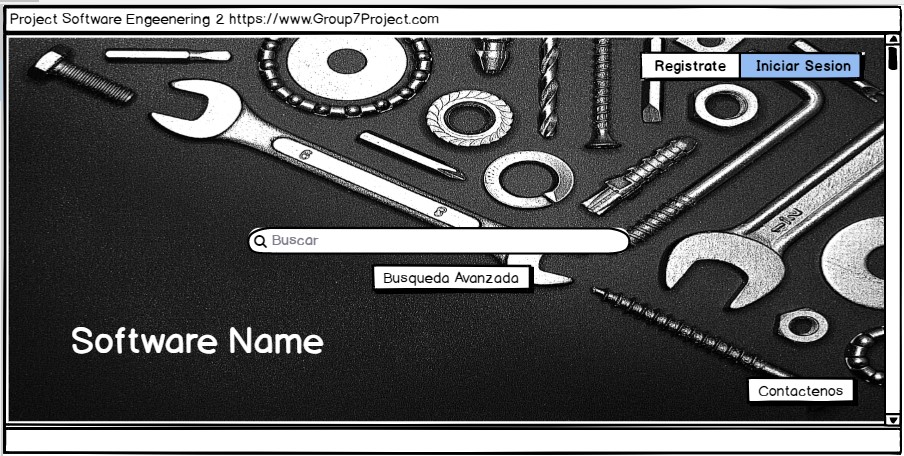
\includegraphics[scale = 0.7]{images/PaginaPrincipal.jpg}
    \caption{Pagina Principal}
    \label{F100}
\end{figure}{}

\begin{figure}[H]
    \centering
    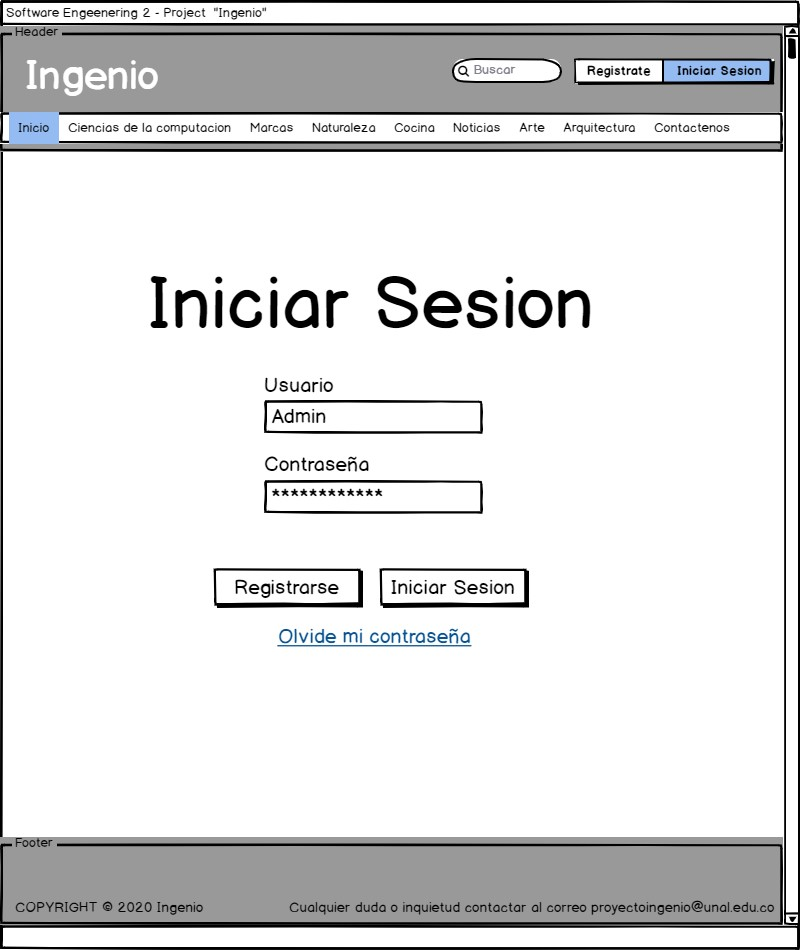
\includegraphics[scale = 0.7]{images/IniciarSesion.jpg}
    \caption{Iniciar Sesión}
    \label{F101}
\end{figure}{}

\begin{figure}[H]
    \centering
    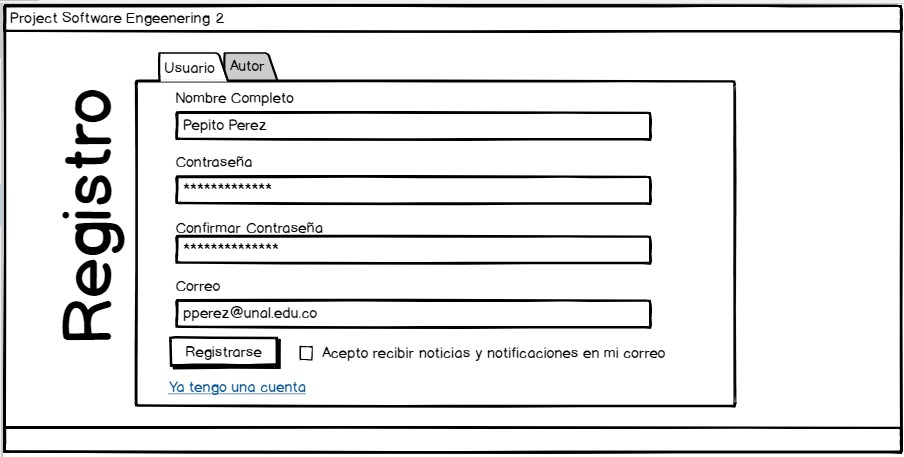
\includegraphics[scale = 0.7]{images/RegistrarseUsuario.jpg}
    \caption{Registrarse Usuario}
    \label{F102}
\end{figure}{}

\begin{figure}[H]
    \centering
    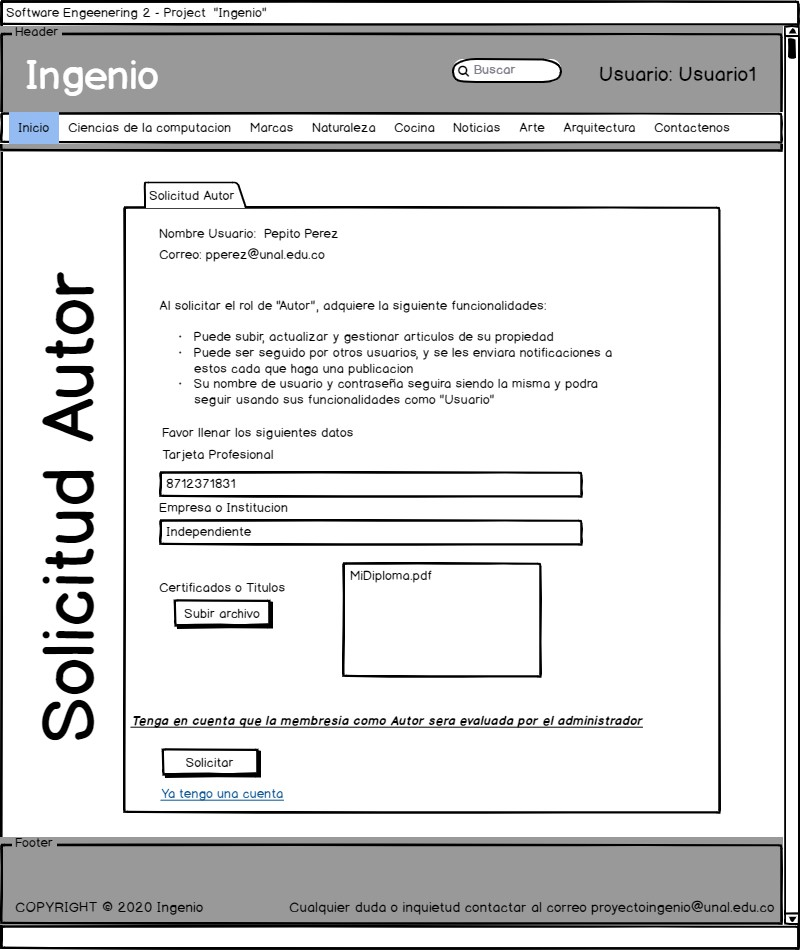
\includegraphics[scale = 0.7]{images/SolicitudAutor.jpg}
    \caption{Solicitud Autor}
    \label{F103}
\end{figure}{}

\begin{figure}[H]
    \centering
    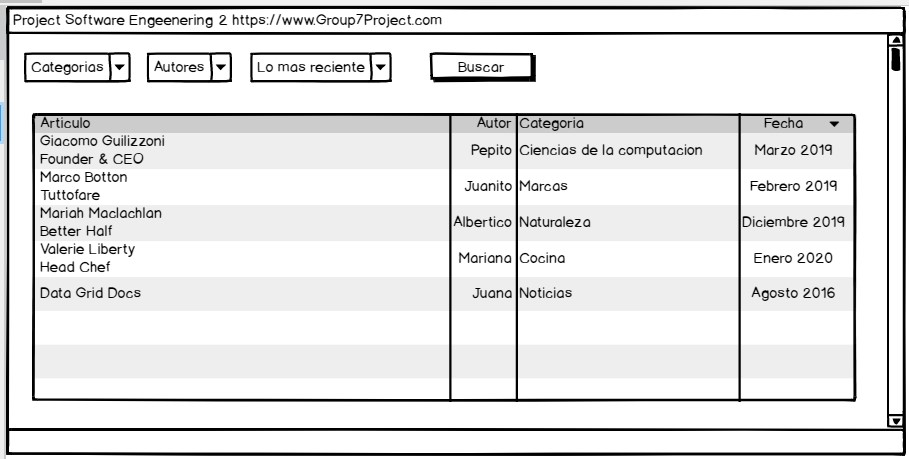
\includegraphics[scale = 0.7]{images/BusquedaAvanzada.jpg}
    \caption{Búsqueda Avanzada}
    \label{F104}
\end{figure}{}

\begin{figure}[H]
    \centering
    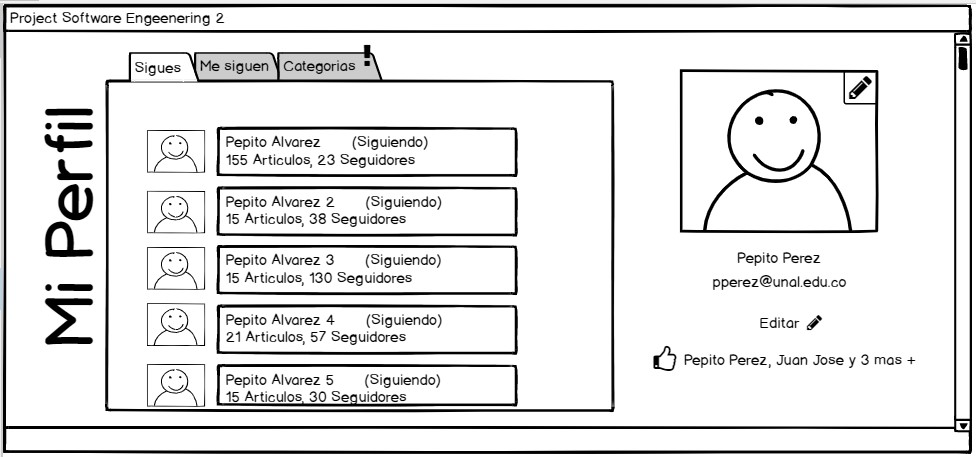
\includegraphics[scale = 0.7]{images/PerfilPropioUsuario.jpg}
    \caption{Perfil Propio Usuario}
    \label{F105}
\end{figure}{}

\begin{figure}[H]
    \centering
    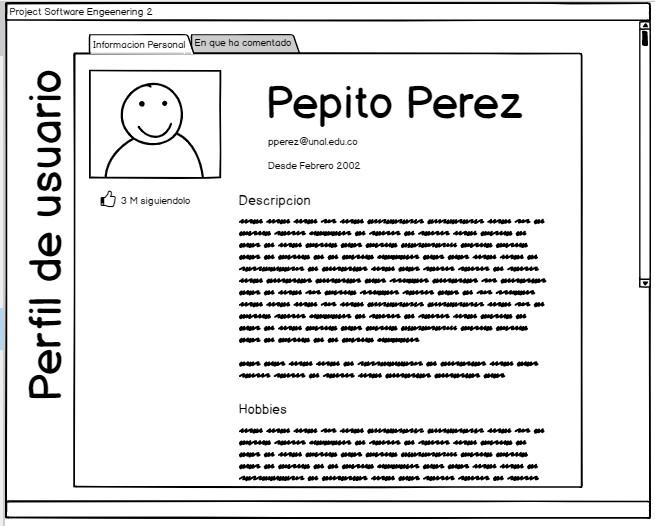
\includegraphics[scale = 0.7]{images/PerfilOtroUsuario.jpg}
    \caption{Perfil Otro Usuario}
    \label{F106}
\end{figure}{}

\begin{figure}[H]
    \centering
    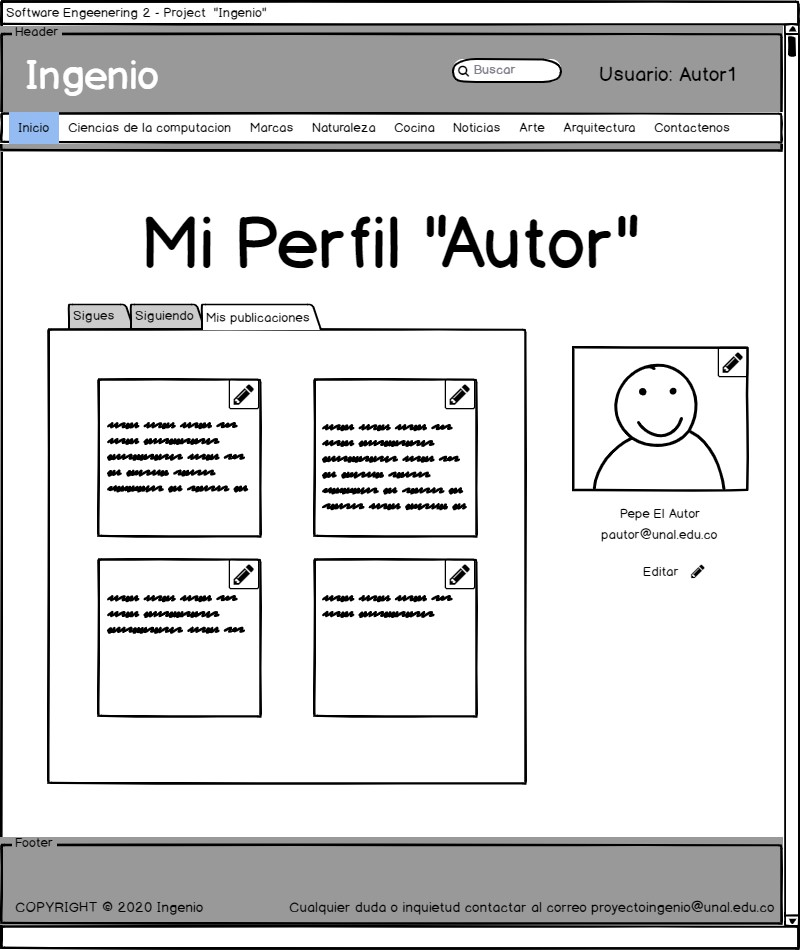
\includegraphics[scale = 0.71]{images/PerfilPropioAutor.jpg}
    \caption{Perfil Propio Autor}
    \label{F107}
\end{figure}{}

\begin{figure}[H]
    \centering
    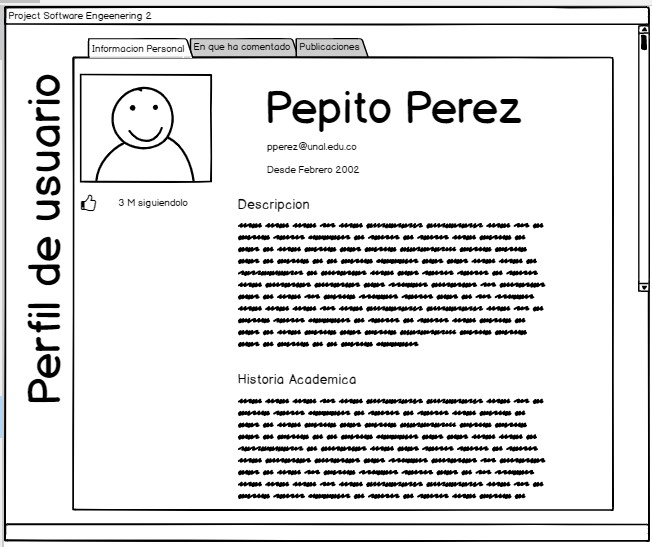
\includegraphics[scale = 0.7]{images/PerfilOtroAutor.jpg}
    \caption{Perfil Otro Autor}
    \label{F108}
\end{figure}{}

\begin{figure}[H]
    \centering
    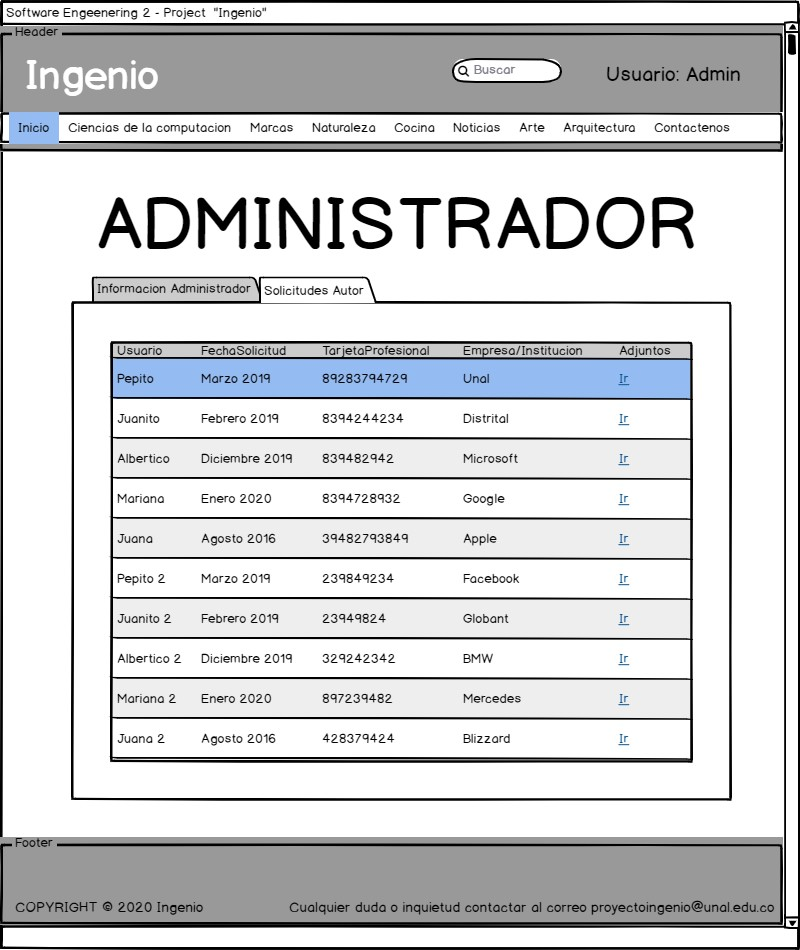
\includegraphics[scale = 0.7]{images/PerfilAdministrador.jpg}
    \caption{Perfil Administrador}
    \label{F109}
\end{figure}{}

\begin{figure}[H]
    \centering
    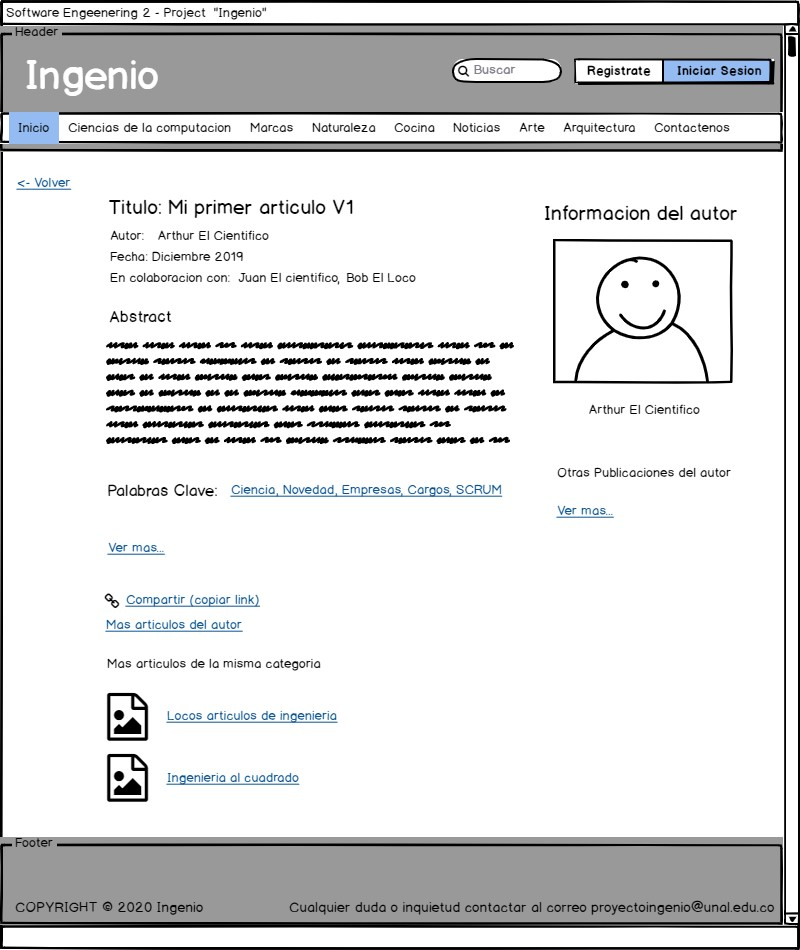
\includegraphics[scale = 0.7]{images/PublicacionVisitante.jpg}
    \caption{Publicación Visitante}
    \label{F110}
\end{figure}{}

\begin{figure}[H]
    \centering
    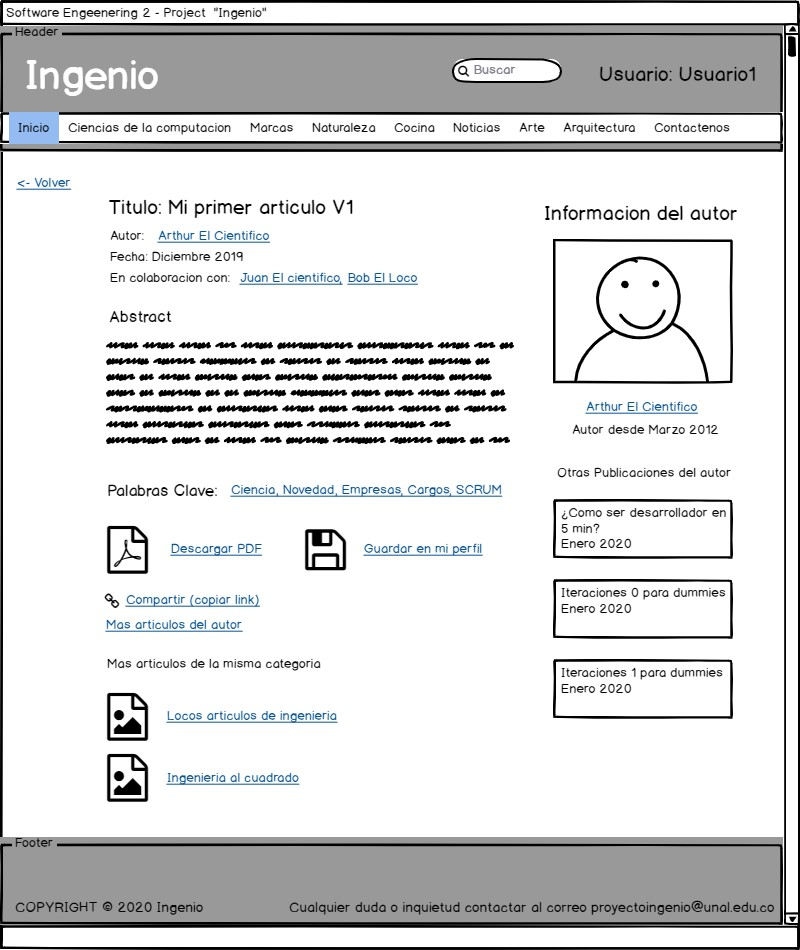
\includegraphics[scale = 0.7]{images/Publicacion.jpg}
    \caption{Publicación}
    \label{F111}
\end{figure}{}

\begin{figure}[H]
    \centering
    
\includegraphics[scale = 0.7]{images/Contactenos.jpg}
    \caption{Contactenos}
    \label{F112}
\end{figure}{}

\begin{landscape}
\section{Modelo Entidad Relación}
    \begin{figure}[H]
        \centering
        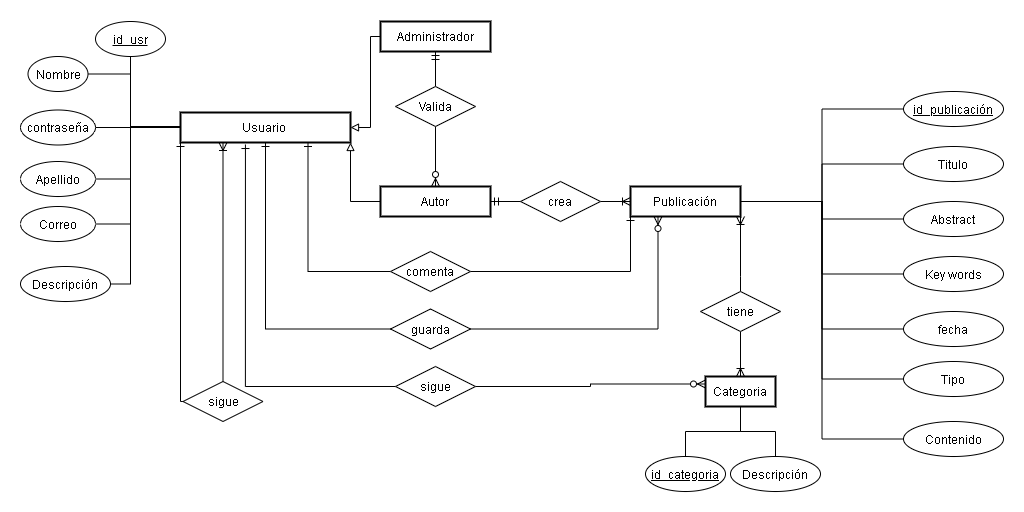
\includegraphics[scale = 0.7]{images/ERD_v02.png}
        \caption{Diagrama modelo ER.}
        \label{F13}
    \end{figure}{}

\section{Modelo de Base de Datos}
    \begin{figure}[H]
        \centering
        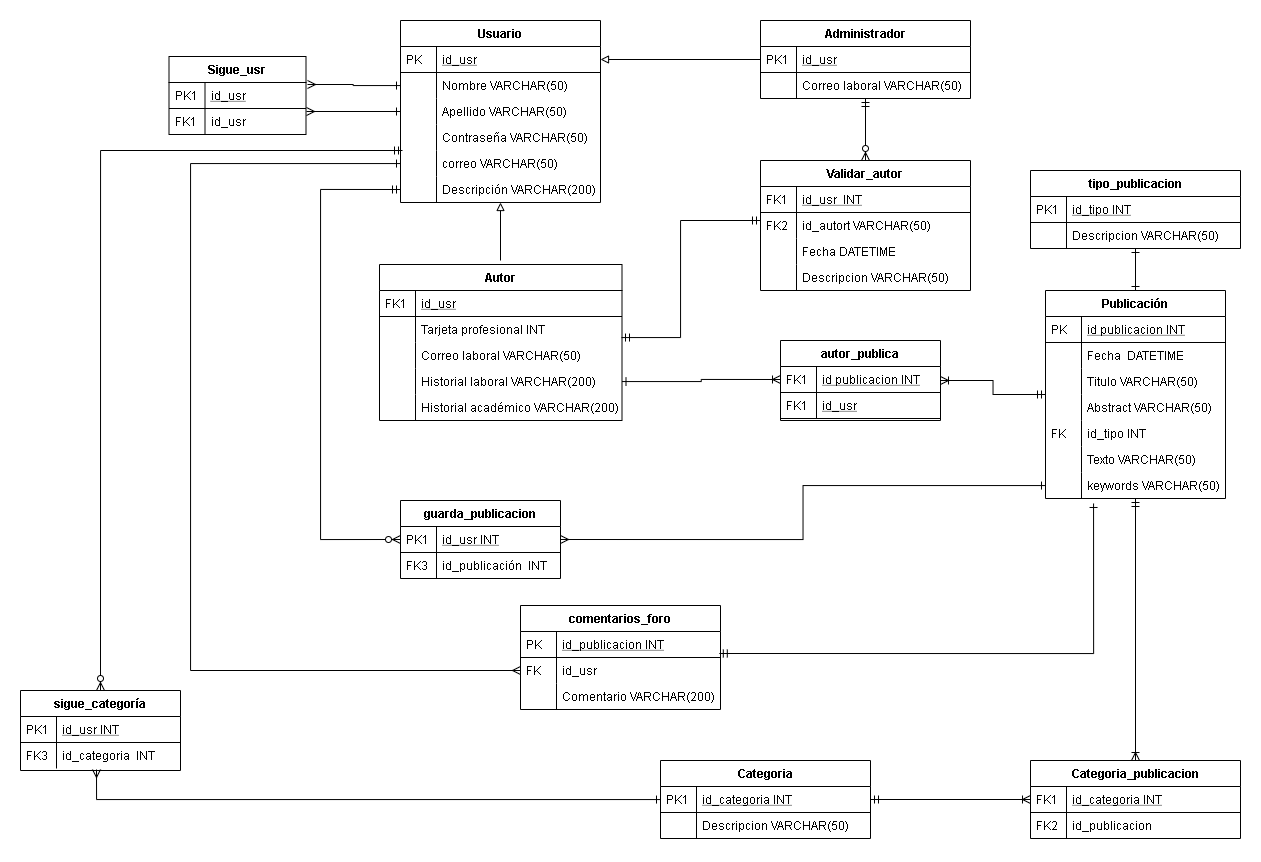
\includegraphics[scale = 0.55]{images/BD_v02.png}
        \caption{Diagrama modelo BD}
        \label{F11}
    \end{figure}{}
\end{landscape}

\section{Estimación de Costos}
El tiempo estimado para realizar el proyecto es del 25 de Marzo del 2020 al 25
de Junio del 2020 (3 meses). \textbf{Por lo tanto todos los gastos se contemplan
para este tiempo estimado}.\\

\textbf{Costos Directos de Personal:}

Los costos directos de personal hacen referencia a las personas contratadas que
colaboran directamente en el proyecto; Scrum Master y 3 desarrolladores.\\

Según la página de búsqueda de empleos “Indeed” \cite{01}, el salario promedio
de un desarrollador de Software en Colombia es de \$ 2’383.039 COP al mes y para
un Scrum Master es de \$3.942.313 .Tanto el Scrum Master, como los
desarrolladores, se encuentran en últimos semestres de universidad, al momento
realizar el proyecto y sus contratos serán al termino de prestación de
servicios. 

% plantilla: copiar y pegar
\begin{table}[H]
    \centering
    \small{
    \begin{tabular}{R{6cm}L{6cm}}
        \textbf{Concepto}   &\textbf{Valor(3 meses)}\\
        \\
        \multicolumn{2}{c}{Scrum master  \dotfill  \$11'826.939} \\
        \multicolumn{2}{c}{Desarrolladores x 3  \dotfill \$21'447.351} \\
        \hline
        \multicolumn{2}{c}{\textbf{Total} \dotfill \$33'274.290} \\
    \end{tabular}
    \label{T04}}
\end{table}{}


\textbf{Costos Indirectos de Personal:}


Los costos indirectos de personal son las personas contratadas que no aportan
directamente al proyecto pero que son necesarias para realizar el trabajo.

Se contratara personal de aseo para hacer la limpieza en la oficina dos veces al
mes, y se le pagara \$ 30.000 COP / día.

\begin{table}[H]
    \centering
    \small{
    \begin{tabular}{R{6cm}L{6cm}}
        \textbf{Concepto}   &\textbf{Valor(3 meses)}\\
        \\
        \multicolumn{2}{c}{Personal de Aseo  \dotfill  \$180.000} \\
        \hline
        \multicolumn{2}{c}{\textbf{Total} \dotfill \$180.000} \\
    \end{tabular}
    \label{T201}}
\end{table}{}

\textbf{Costos Directos de Material:}

Estos costos son los relacionados a la compra o alquiler de equipos necesarios 
para el desarrollo del software, para este proyecto consideramos el alquiler de 
4 computadores \cite{02} por un valor mensual de \$220.000 COP / cada uno,
además se consideran 
el consumo de internet y energía eléctrica en el lugar de desarrollo, estos
corresponden a un valor de \$110.000 COP/mensual de servicio 
de energía eléctrica y \$103.000 COP / mensual por servicio de internet, también
se contempla la compra de mueblería a usar, que consta de 4 escritorios y 4
sillas, por valor de \$2'000.000 COP.

\begin{table}[H]
    \centering
    \small{
    \begin{tabular}{R{6cm}L{6cm}}
        \textbf{Concepto}   &\textbf{Valor(3 meses)}\\
        \\
        \multicolumn{2}{c}{Alquiler de equipos x 4  \dotfill  \$2'640.000} \\
        \multicolumn{2}{c}{Servicio de energía eléctrica\dotfill  \$330.000} \\
        \multicolumn{2}{c}{Servicio de internet \dotfill \$309.000} \\
        \multicolumn{2}{c}{Compra Mueblería \dotfill \$2'000.000} \\
        \hline
        \multicolumn{2}{c}{\textbf{Total} \dotfill \$5'279.000} \\
    \end{tabular}
    \label{T03}}
\end{table}{}

\textbf{Costos Indirectos de Material:}

Estos costos son los no relacionados directamente con el proyecto, pero
necesarios en el ambiente de trabajo. Tales como, recibo de agua por un valor
mensual de \$120.000 COP, además implementos de aseo que corresponden a un valor
de \$150.000 COP/mensual y gastos varios o de papelería por \$50.000 COP /
mensual.

\begin{table}[H]
    \centering
    \small{
    \begin{tabular}{R{6cm}L{6cm}}
        \textbf{Concepto}   &\textbf{Valor(3 meses)}\\
        \\
        \multicolumn{2}{c}{Servicio de agua \dotfill  \$360.000} \\
        \multicolumn{2}{c}{Implementos de aseo 
        \dotfill  \$450.000} \\
        \multicolumn{2}{c}{Papelería y varios
        \dotfill \$150.000} \\
        \hline
        \multicolumn{2}{c}{\textbf{Total} \dotfill \$960.000} \\
    \end{tabular}
    \label{T203}}
\end{table}{}

\textbf{Total de Costos:}

En esta sección se encuentra el resumen de todos los costos del proyecto, y el
valor final a cobrar.

\begin{table}[H]
    \centering
    \small{
    \begin{tabular}{R{6cm}L{6cm}}
        \textbf{Concepto}   &\textbf{Valor(3 meses)}\\
        \\
        \multicolumn{2}{c}{Costos directos personal  \dotfill  \$33'274.290} \\
        \multicolumn{2}{c}{Costos indirectos personal  \dotfill  \$180.000} \\
        \multicolumn{2}{c}{Costos directos de material \dotfill \$5'279.000} \\
        \multicolumn{2}{c}{Costos indirectos de material \dotfill \$960.000} \\
        \hline
        \multicolumn{2}{c}{\textbf{Total (antes de instalación)} 
        \dotfill \$39'693.290} \\
        \multicolumn{2}{c}{Instalación \dotfill \$500.000} \\
        \hline
        \multicolumn{2}{c}{\textbf{Total (antes de ganancia esperada)} 
        \dotfill \$40'193.290} \\
        \multicolumn{2}{c}{Ganancia esperada (20\%) \dotfill \$8'038.658} \\
        \hline
        \multicolumn{2}{c}{\textbf{Total (Precio mínimo)} 
        \dotfill \$48'231.948} \\
        \multicolumn{2}{c}{Ajuste Final \dotfill - \$231.948} \\
        \hline
        \multicolumn{2}{c}{\textbf{Total Esfuerzo Nominal} 
        \dotfill \$48'000.000} \\
        \multicolumn{2}{c}{Esfuerzo de sobrecarga (50\%) 
        \dotfill - \$24'000.000} \\
        \hline
        \multicolumn{2}{c}{\textbf{Costo Total} \dotfill \$72'000.000} \\
    \end{tabular}
    \label{T205}}
\end{table}{}

Se estima un valor total \$72'000.000 COP por el costo total del proyecto.


\section{Análisis de riesgos}


\begin{table}[H]
    \centering
    \small{
    \begin{tabular}{|M{1cm}|M{3cm}|M{10cm}|}
        \hline
        \textbf{Valor}  &\textbf{Tipo}   &\textbf{Definición}\\
        \hline 
            1   & Técnico
            & Daños o problemas con los dispositivos que intervienen en el
            desarrollo de la aplicación.\\
        \hline
            2  & Organizacional
            & Errores en la ejecución de diferentes planes de trabajo por parte
            de los individuos que intervienen en el desarrollo de la aplicación.
            \\
        \hline
            3   & Cronograma
            & Contratiempos que afectan el desarrollo de actividades en el
            tiempo estimado.      \\
        \hline
            4   & Externo
            & Problemas que son ajenos a la organización.    \\
        \hline
            5   & Gerencial
            & Malas prácticas que provocaron la creación de modelos de trabajo
            inadecuados para el desarrollo de la aplicación.   \\
        \hline
    \end{tabular}
    \caption{Tipos de riesgo}
    \label{Riesgo3}}
\end{table}{}


\begin{table}[H]
    \centering
    \small{
    \begin{tabular}{|M{1cm}|M{2cm}|M{11cm}|}
        \hline
        \textbf{Valor}   &\textbf{Significado}   &\textbf{Criterio}\\
        \hline 
            1   & Muy bajo
            & No afecta el desarrollo, calidad o esencia de la aplicación, ni
            altera el tiempo de ejecución estimado para las siguientes etapas de
            trabajo.\\
        \hline
            2   & Bajo
            & Afecta en pequeña medida la esencia, calidad de la aplicación o el
            cronograma predefinido para cada fase de desarrollo. \\
        \hline
            3   & Moderado
            & Afecta en una medida considerable el cronograma predefinido de
            desarrollo, la calidad de la aplicación o su esencia.  \\
        \hline
            4   & Alto
            & Afecta en gran medida el desarrollo de la aplicación y es
            necesario y redefinir modelos de trabajo para continuar con el
            proyecto.      \\
        \hline
            5   & Muy alto
            & El impacto sobre el cronograma o la aplicación es muy alta y es
            imposible crear un modelo de trabajo que permita retomar el trabajo
            con los recursos disponibles.\\
        \hline
    \end{tabular}
    \caption{Niveles de Impacto}
    \label{Nimpacto}}
\end{table}{}

\small{
\centering
\begin{longtable}{|M{4cm}|M{1cm}|M{1.5cm}|M{2.5cm}|M{6cm}|}
    \endfirsthead
    \multicolumn{5}{c}%
    {{\tablename\ \thetable{} -- Continúa de la página anterior}} \\
    
    \hline
    \textbf{Riesgo} & \textbf{Tipo} &\textbf{Impacto}
    & \textbf{Probabi-lidad} & \textbf{Plan de acción}\\
    \hline
    \endhead
    
    \hline
    \multicolumn{5}{c}{{\tablename\ \thetable{} -- Continúa en la siguiente
    página.}} \\ 
    \endfoot
    \endlastfoot
    
    \hline
    \textbf{Riesgo} & \textbf{Tipo} &\textbf{Impacto}
    & \textbf{Probabilidad} & \textbf{Plan de acción}\\
    \hline
    Un integrante del equipo de desarrollo renuncia.
    & 4 & 3  & 10\%  
    & Distribuir el trabajo del desarrollador entre los
    demás miembros del equipo y evaluar si es necesario replantear la
    entrega prevista.\\
    \hline
    Perdida de herramientas de comunicación de desarrollo tales como internet.
    & 4 &  4 &   4\%
    &  Entrega de paquetes de avance de trabajo periódicamente y coordinado por
    cualquier otro medio de comunicación. \\
    \hline
    El hardware del equipo no cumple con los requerimientos mínimos para
    culminar el desarrollo del proyecto.
    & 3 & 3  & 5\%  
    & Se buscara un hardware que solucione esta necesidad para la culminación
    del proyecto . \\
    \hline
    La planificación del desarrollo de historias de usuario no están bien
    coordinadas.
    & 2 &  4 & 15\%  
    &  Programar las tareas de desarrollo\\
    \hline
    Una tarea requiere mas tiempo de lo esperado.
    & 3 &  3 & 17\%   
    &  Destinar mas horas de trabajo y equipo de  desarrollo para terminar la
    tarea. \\
    \hline
    El proyecto es cancelado por motivos extracurriculares
    & 4 & 5  & 6\%  
    &  Decidir si culminar o no el proyecto \\
    \hline
    La metodología de desarrollo no ofrece el desempeño esperado.
    & 5 & 2  & 15\%
    &  Dado el caso se repensara la implementación de cierta metodología para
    próximos proyectos.  \\
    \hline
    El software presenta errores tiempo después de haber sido completado en
    iteraciones anteriores.
    & 1 & 3  & 30\%  
    & Se hará una revisión de los cambios hasta donde no ocurrían los errores
    solucionados o se decidirá corregirlos juntamente con los cambios realizados
    \\
    \hline
    El scrum master no cumple con lo requerido para mantener al equipo de
    desarrollo activo y entorno saludable.
    & 2 & 1  &  15\%
    &  Cambio del scrum master por algún otro integrante del equipo  \\
    \hline
    Los tiempos de entrega se ven reducidos
    & 3 &  4 & 5\%  
    &  Reprogramación de tareas por cada historia de usuario restante \\
    \hline
    Cambio de objetivo del proyecto por parte del cliente
    & 4 & 5  & 15\%  
    & Replanteamiento de historias de usuario y buscar homologación del trabajo
    realizado  \\
    \hline
    Priorización inadecuada en la gestión de proyectos.
    & 5 & 2  & 20\%
    & Buscar nuevas formas de organizar las tareas en siguientes iteraciones. \\
    \hline
    \caption{Riesgos de desarrollo.} 
    \label{Riesgos}
\end{longtable}}


\section {Comparación Frameworks }

Para la elección de Frameworks que serán usados en el desarrollo del proyecto se realizo una comparación, entre diferentes entornos de trabajo tanto para Back End y Front End, considerando: su popularidad, la disponibilidad de recursos de aprendizaje y sus funciones principales, mostrando sus ventajas y desventajas.\\

\textbf{FrontEnd}:\\

Para la elección de frameworks en FrontEnd se tuvo en cuenta, \textbf{React}, \textbf{Angular} y \textbf{Vue}.\\

Inicialmente fueron considerados estos tres entornos dada su popularidad, ya que son de las herramientas más usadas en la actualidad, por lo tanto cuentan con una gran comunidad de desarrolladores, lo cual nos permite contar con mayor información y dada la antigüedad de algunos, se podría tener mas oportunidades en el ámbito laboral (React y Angular), en la siguiente tabla se muestra la información correspondiente a la popularidad de estos entornos. 

\begin{table}[H]
    \centering
    \small{
    \begin{tabular}{|M{5cm}|M{2.5cm}|M{2.5cm}|M{2.5cm}|}
        \hline
         &\textbf{Angular}   &\textbf{React} &\textbf{Vue Js}\\
        \hline 
            Stars on GitHub   & 26,924
        & 73,530 & 63,438
            \\
        \hline
            Contributors on GitHub & 495
        & 1044 & 122
            \\
        \hline
            Tagged questions on StackOverflow  & 66,152
        & 54,158 & 8598
            \\
        \hline
    \end{tabular}
    \caption{Popularidad, Tomado de \cite{03}}
    \label{Riesgo}}
\end{table}{}

Respecto a las funciones principales, todas tiene características que permiten destacar cada una de las herramientas; como por ejemplo Angular,que permite desde su entorno trabajar procesamiento y validación de formularios y comunicación HTTP, por el contrario estas son tareas que en React y Vue dependen del desarrollador, a continuación se muestra una tabla con las ventajas y desventajas de cada Framework.

\begin{table}[H]
    \centering
    \small{
    \begin{tabular}{|M{2.5cm}|M{6.5cm}|M{6.5cm}|}
        \hline
        \textbf{Framework}  &\textbf{Ventajas}   &\textbf{Desventajas}\\
        \hline 
            React   &
            \begin{itemize}
                \item Alto desempeño.
                \item Adecuado para aplicaciones con mucho tráfico.
                \item DOM virtual(enlace de datos unidireccional).
            \end{itemize}   &
            \begin{itemize}
                \item Necesita otras librerías para construir aplicaciones complejas.
            \end{itemize}
            \\
        \hline
            Angular & 
            \begin{itemize}
                \item Enlace de datos bidireccional
                \item Aplicación simple de una pagina.
                \item Permite procesamiento y validación de formularios.

            \end{itemize}   &
            \begin{itemize}
                \item Se debe aprender Typescript.
                \item Complejo y difícil de aprender.
            \end{itemize}
            \\
        \hline
            Vue.js  & 
            \begin{itemize}
                \item Alto desempeño. 
                \item Flexibilidad. 
                \item DOM visual y basado en componentes
            \end{itemize}   &
            \begin{itemize}
                \item El más joven del los entornos 
                \item Poco mercado.
                \item Ser demasiado flexible puede generar problemas
            \end{itemize}
            \\
        \hline
            
    \end{tabular}
    \caption{Frameworks FrontEnd}
    }
\end{table}{}

Considerando la información anterior, seleccionamos Vue JS como framework FrontEnd, ya que es uno de los más fáciles de aprender y se adapta fácilmente en la creación de interfaces de usuario además proporciona un período de cambio rápido de otros frameworks a Vue.js debido a la similitud con Angular y React en términos de diseño y arquitectura.\\

\textbf{BackEnd}:\\

Para realizar la comparacion de frameworks en Back End, decidimos analizar algunos de los mas usados y conocidos actualmente, \textbf{Sprint (Java)}, \textbf{Django (Python)} y \textbf{Node JS (Javascript)}.\\


\begin{table}[H]
    \centering
    \small{
    \begin{tabular}{|M{2.5cm}|M{6.5cm}|M{6.5cm}|}
        \hline
        \textbf{Framework}  &\textbf{Ventajas}   &\textbf{Desventajas}\\
        \hline 
            Spring   & 
            \begin{itemize}
                \item Buena separación entre componentes de front-end y la lógica de Java.
                \item Desarrollo orientado a componentes estilo SWING
                \item Facil de debuggear
                \item Su uso son Java y HTML simples, los conceptos de Java se utilizan a gran nivel
            \end{itemize}   & 
            \begin{itemize}
                \item Se actualiza muy constantemente, y esto puede causar problema con versiones nuevas
                \item Entre mas componentes tiene una pagina, mas complejo y desorganizado se vuelve el codigo
                \item Limitado a pagina simples
                \item Documentacion actalizada escaza
            \end{itemize}
            \\
        \hline
            Django & 
            \begin{itemize}
                \item Django fue creado para trabajar bajo un patrón MVC (Modelo Vista Controlador) quien se encarga del manejo de controladores, esto lo caracteriza en un framework reusable y permite el desarrollo ágil.
                \item Según la comunidad que desarrolla bajo Python, los API’s REST que genera Django son mucho mejores, debido a que se pueden convertir en páginas HTML como puntos finales (Endpoints).
                \item Tiene un panel de administración para gestionar bases de datos.
            \end{itemize}   &
            \begin{itemize}
                \item A pesar de su excelente documentación, es muy extensa y tiende a ser confusa.
                \item A la hora de realizar un API REST conlleva cierta condición de dificultad a comparación de Flask.
                \item La implementación de sockets es algo compleja de usar.
            \end{itemize}
            \\
        \hline
            Node.js  &
            \begin{itemize}
                \item Si tu aplicación no tiene ningún cálculo intensivo del CPU, puedes construir en Javascript de arriba a abajo, inclusive a nivel de base de datos si utilizas el objeto de almacenamiento JSON como MongoDB DB. Esto facilita el desarrollo (incluyendo la contratación) significativamente.
                \item Los Crawlers reciben una respuesta totalmente HTML, que es mucho más SEO-friendly, digamos, una sola página o en una aplicación de Websockets app se ejecuta sobre Node.js.
            \end{itemize}   &
            \begin{itemize}
                \item • Un CPU de cálculo intensivo bloqueará la receptividad del Node.js, por lo que una plataforma de roscado es un mejor enfoque. Alternativamente, podrías intentar escalar el cómputo.
                \item • Utilizando Node.js con una base de datos relacional es aún bastante doloroso (leer más abajo para ver más detalles). Hazte un favor y escoge cualquier otro entorno como Rails, Django, o ASP.NET MVC si estás intentando realizar operaciones relacionales.
            \end{itemize}
            \\
        \hline
            
    \end{tabular}
    \caption{Frameworks BackEnd}
    }
\end{table}{}

Segun la comparacion de estos tres llegamos a la eleccion de \textbf{NODE JS}.\\

Ya que la eleccion para Front End fue  Vue JS, recurrimos a la tarea de analizar los Stacks mas usados y pedidos dentro de la industria de software que se relacionaran de mejor manera a estos frameworks.\\

Al buscar esto, encontramos que los mas usados son:\\ 

\textbf{Stack MEAN}:

MongoDB, Express, AngularJS y Node.js\\

\textbf{Stack MERN}:

MongoDB, Express, React y Node.js\\

Lo que nos llevo a encontrar:

\textbf{Stack MEVN}:

MongoDB, Express, Vue y Node.js\\


El cual funciona de la siguiente forma:
\begin{itemize}
\item MongoDB: servicio de gestión de bases de datos multiplataforma orientado a documentos (conjunto de registros o de datos) y de esquema totalmente libre (no debe estar predefinido). Así, cada documento puede tener atributos distintos al resto.
\item Vue JS: marco de desarrollo de front-end. Es un framework de JavaScript de código abierto y libre, que permite el desarrollo de aplicaciones web en el lado del cliente.
\item Node.js: entorno de desarrollo en la capa del servidor. Su objetivo es que un programador sea capaz de desarrollar una aplicación con altos niveles de escalabilidad en una única máquina, aunque las peticiones de usuarios y clientes no dejen de aumentar con el tiempo.  La lógica apunta a la fórmula ‘más clientes, más coste’, pero Node.js rompe esa ecuación.
\item Express: framework para el desarrollo de back-end. Es un marco de desarrollo rápido, flexible y con una gran comunidad detrás, lo cual siempre es importante por el volumen de documentación existente para el desarrollo de proyectos.
\end{itemize}

Y este el ultimo \textbf{sera el Stack que se usara para realizar el desarrollo} de "Ingenio". Otro factor importante para la eleccion de este Stack, es la programacion usando un solo lenguaje (Javascript) tanto para Front End y Back End.

%%%Escribir justificacion
\section{Repositorio }

\begin{itemize}
    \item BackEnd
    \item FrontEnd
\end{itemize}

\section{Sprint 1}

\section*{Tablero Kanban}
\section*{Slack} 
\section*{Hash Spritn 1}
\begin{itemize}
    \item BackEnd
    \item FrontEnd
\end{itemize}


\begin{thebibliography}{50}

\bibitem{01} Indeed Salarios. \\
Disponible en: 
\url{https://co.indeed.com/salaries/desarrollador-de-software-Salaries}

\bibitem{02} Renta sistemas.\\
Disponible en:
\url{https://www.rentasistemas.com/}

\bibitem{03}Adictec, Cómo Elegir el Mejor Framework de Front-End.\\
Disponible en:
\url{https://adictec.com/como-elegir-el-mejor-framework-de-front-end/}

\bibitem{04}Angular.\\
Disponible en:
\url{https://angular.io/docs}

\bibitem{05}Vue Js.\\
Disponible en:
\url{https://vuejs.org/}

\bibitem{06}React.\\
Disponible en:
\url{https://es.reactjs.org/docs/getting-started.html}

\bibitem{07}Which front-end framework is the best in 2019.\\
Disponible en:
\url{https://www.blog.duomly.com/which-front-end-framework-is-the-best-in-2019}

\bibitem{08}Which front-end framework is the best in 2019.\\
Disponible en:
\url{https://medium.com/drakezair/reactjs-vs-angularjs-vs-vuejs-la-pelea-de-los-grandes-2018-5f4027e61cef}

\bibitem{09} ¿Por qué demonios usaría Node.js? Un tutorial caso por caso\\
Disponible en 
\url{https://www.toptal.com/nodejs/por-que-demonios-usaria-node-js-un-tutorial-caso-por-caso}

\bibitem{10} ¿Porqué alguien usaría JavaScript para el backend?\\
Disponible en 
\url{https://medium.com/fixtergeek/porqu%C3%A9-alguien-usar%C3%ADa-javascript-para-el-backend-e48442d9b561}

\bibitem{11} ¿Cuál es el stack tecnológico más popular?\\
Disponible en 
\url{https://www.syntonize.com/stack-tecnologico-mas-popular/}

\bibitem{12} Qué es el stack MEAN y cómo escoger el mejor para ti\\
Disponible en 
\url{https://www.campusmvp.es/recursos/post/Que-es-el-stack-MEAN-y-como-escoger-el-mejor-para-ti.aspx}

\end{thebibliography}{}
\end{document}{}

\bibitem{04}Angular. Disponible en:\url{https://angular.io/docs}

\bibitem{05}Vue Js.
Disponible en:\url{https://vuejs.org/}

\bibitem{06}React.
Disponible en:\url{https://es.reactjs.org/docs/getting-started.html}

\bibitem{07}Which front-end framework is the best in 2019, 
Disponible en:\url{https://www.blog.duomly.com/which-front-end-framework-is-the-best-in-2019}
\bibitem{08}Which front-end framework is the best in 2019, 
Disponible en:\url{https://medium.com/drakezair/reactjs-vs-angularjs-vs-vuejs-la-pelea-de-los-grandes-2018-5f4027e61cef}

\end{thebibliography}{}
\end{document}{}
